%----------------------------------------------------------------------------------------
%	PACKAGES AND THEMES
%----------------------------------------------------------------------------------------

\documentclass[aspectratio=169,xcolor=table]{beamer}

%Cheat-Sheet: https://www.cpt.univ-mrs.fr/~masson/latex/Beamer-appearance-cheat-sheet.pdf

%-- Layout --%
% font size
\usepackage[fontsize=11pt]{scrextend}
\usepackage{amsmath}
\usepackage{lscape} % or pdflscape for PDF output
\usepackage{tcolorbox}
\usepackage{appendixnumberbeamer} 
\usepackage[short]{optidef}
\usepackage[backend=bibtex,style=authoryear]{biblatex}
\usepackage{tabularx}
\usepackage{booktabs}
\usepackage{colortbl}
% \usepackage[table]{xcolor}  % loaded by beamer (class option xcolor=table)
% for the indicator function
% page

\setbeamersize{text margin left=1cm, text margin right=1cm}
\setbeamercolor{button}{bg=blue, fg=white}
% line space 
% footline
\addtobeamertemplate{navigation symbols}{}{
    \usebeamerfont{footline}
    % \usebeamercolor[fg]{footline}
    \hspace{2em}
    \insertframenumber/\inserttotalframenumber    }
% headline
\setbeamercovered{transparent}
\setbeamertemplate{itemize item}{\raisebox{0.2ex}{\small\textbullet}}
\setbeamertemplate{itemize subitem}{--} % Second level

\usetheme[progressbar=frametitle]{metropolis}

\makeatletter
\setlength{\metropolis@titleseparator@linewidth}{1.25pt}
\setlength{\metropolis@progressonsectionpage@linewidth}{1.25pt}
\setlength{\metropolis@progressinheadfoot@linewidth}{1.25pt}
\makeatother

\setbeamertemplate{frame numbering}[fraction]
\setbeamercovered{invisible}

\definecolor{primary}{RGB}{0, 150, 255}
\setbeamercolor{palette primary}{bg=white, fg=black}
\setbeamercolor{background canvas}{parent=palette primary}
\setbeamercolor{normal text}{fg=black}
\setbeamercolor{progress bar}{use=palette primary,fg=primary}

%-- Figure --%
\usepackage{graphicx}
% \usepackage{subfig}

\DeclareMathOperator*{\argmin}{arg\,min} % Jan Hlavacek
\DeclareMathOperator*{\argmax}{arg\,max} % Jan Hlavacek
\DeclareMathOperator{\E}{\mathbb{E}}
\def\boxit#1{%
  \smash{\color{red}\fboxrule=1pt\relax\fboxsep=2pt\relax%
  \llap{\rlap{\fbox{\vphantom{0}\makebox[#1]{}}}~}}\ignorespaces
}

%-- Table --%
\usepackage{tabularx,booktabs}
\newcolumntype{Y}{>{\centering\arraybackslash}X}

%-- Text --%
% \usepackage{xcolor}  % loaded by beamer (class option xcolor=table)

% \usepackage{tikz}

%-- Math --%
\usepackage{amssymb}
\usepackage{amsmath}
\usepackage{enumitem}

%-- Caption --%
\usepackage{caption}
\usepackage{subcaption}

%-- Effects --%
\usepackage{hyperref}
\hypersetup{
    colorlinks=true,
    linkcolor=blue,         % Color of internal links
    filecolor=blue,         % Color of file links
    urlcolor=blue}

\newcommand{\smallbullet}{\raisebox{0.3ex}{\scalebox{0.7}{$\bullet$}}}


%----------------------------------------------------------------------------------------
%	TITLE PAGE
%----------------------------------------------------------------------------------------
\title[]{Bankruptcy Resolution and the Macroeconomics \\ of Cash Flow-Based Lending} % The short title appears at the bottom of every slide, the full title is only on the title page

\author{Barnab\'as Sz\'ekely} % Your name

\date{\today } % Date, can be changed to a custom date

\providecommand{\E}{\mathbb{E}}
\providecolor{lightblue}{RGB}{235,245,255}
\begin{document}
\renewcommand{\arraystretch}{1.4}
\setlist[itemize]{label=\smallbullet, noitemsep, topsep=0pt, parsep=0pt, partopsep=0pt}

\begin{frame}
\titlepage % Print the title page as the first slide
\end{frame}

%%----------------------------------------------------------------------------------------
%	PRESENTATION SLIDES
%---------------------------------------------------------------------------------

%---------------------------------------------------------------------------------
\begin{frame}[label=motivation1]
    \frametitle{Motivation}

Credit constraints are major impediments to firm growth \hfill \footnotesize - Beck et al. (2006)
\begin{itemize} \small
    \item Typically attributed to a lack of physical collateral 
\end{itemize} \normalsize  \vspace{4mm}

Most of corporate debt is backed by future cash flows rather than assets       \hfill \hyperlink{LandM}{\beamergotobutton{Details}}
\begin{itemize} \small
    \item \textbf{Cash flow-based} borrowing could relax collateral constraints for asset-poor firms 
\end{itemize} \normalsize  \vspace{5mm}

\pause

However, cash flow-based debt remains expensive for most firms  \hfill \hyperlink{spreads}{\beamergotobutton{Visually}}
 
 \footnotesize
 \begin{table}[h]
    \centering
    \renewcommand{\arraystretch}{1}
    \begin{tabular}{lcc}
        \hline
       \textbf{Credit Spread} & \multicolumn{2}{c}{\textbf{Total Asset Value}} \\ 
         &  $\leq$ 100M USD  &  $>$ 100M USD \\
        \hline
        Cash flow-based debt  & 7.19\%  & 3.12\%  \\
        Asset-based debt  & 5.25\%  & 3.93\%  \\
         \hline
         & \multicolumn{2}{c}{ \hfill \textit{\scriptsize Source: Compustat, CapitalIQ \normalsize}} \\
    \end{tabular}
    \label{tab:credit_spread}
\end{table}


\end{frame}

%---------------------------------------------------------------------------------
\begin{frame}[label=motivation2]
    \frametitle{Motivation}

 Probability of liquidation in default decreases with firm size  \hfill \hyperlink{liqprob}{\beamergotobutton{Data}}
 \footnotesize 
 \begin{table}[h]
    \centering
    \renewcommand{\arraystretch}{1}
    \begin{tabular}{lcc}
        \hline
        \textbf{Total Asset Value} &  \textbf{$\leq$ 100M USD}  &  \textbf{$>$ 100M USD} \\
        Share Liquidated  & 76.7\%  & 7.61\%   \\
        \hline
        & \multicolumn{2}{c}{ \hfill \textit{\scriptsize Source: FJC Integrated Database \normalsize}} \\
    \end{tabular}
    \label{tab:credit_spread}
\end{table} \normalsize \vspace{-1mm}

Large \textbf{reorganization costs} often force the liquidation of small firms  \hfill \hyperlink{FCreorg}{\beamergotobutton{Details}} \vspace{3mm} \\


Liquidation (exit) terminates all future cash flows 
\begin{itemize}  \small
    \item Cash flow-based debt: lenders must offset liquidation risk by imposing higher spreads
\end{itemize} \normalsize  \vspace{3mm}

\pause

In this paper, I ask:
\begin{itemize}\small
    \item[1.] How do reorganization costs limit `small' firms' access to cash flow-based debt?
    \item[2.] How does this affect firm dynamics and aggregate outcomes?
\end{itemize}

\end{frame}


%------------------------------------------------
\begin{frame}[label=What I do] \frametitle{What I do}

I develop \textbf{a general equilibrium model} featuring,
\begin{itemize} 
    \item Heterogeneous firms with endogenous borrowing decisions and default
    \item Two types of debt contracts and default resolution  \vspace{1mm}
\begin{itemize} \small
    \item Asset-based vs. Cash flow-based debt 
    \item Liquidation vs. Reorganization, subject to \textbf{fixed costs}  
\end{itemize}
\end{itemize} \normalsize  \vspace{3mm}

\textbf {Calibrated} to U.S non-financial corporations (2010 - 2024)  \vspace{3mm} \\
\textbf{Contributions}
\begin{itemize} \small
    \item[1.] Evaluate the GE effects of a reduction of reorganization costs
   \item[2.] Evaluate recent bankruptcy reforms (U.S. SBRA; EU Reorganization Directive)
\end{itemize}

\end{frame} 


%------------------------------------------------
\begin{frame}[label=lit] \frametitle{Related Literature \& \textcolor{red}{Contribution} }

\textbf{Heterogeneous firms and credit market frictions}: \\
\footnotesize \textit{Khan and Thomas (2013), Khan Senga and Thomas (2020), Azariadis, Kaas and Wen (2016), \\ Corbae and D'Erasmo (2021), Ottonello and Winberry (2020), Kochen (2022)} \normalsize \\ 
\qquad $\Rightarrow$ \textcolor{red}{Heterogeneity of debt contract and default resolution} \vspace{3mm} \\

\textbf{Heterogeneous debt contracts and borrowing constraint}: \\
\footnotesize \textit{Drechsel (2023), Choi (2022), Lian and Ma (2021), Ivashina, Laeven, Moral-Benito (2020), Drechsel and Kim (2022), Öztürk (2023), Caglio, Darst and Kalemli-Ozcan (2021), González and Sy (2024)} \normalsize \\ 
\qquad $\Rightarrow$ \textcolor{red}{In equilibrium defaults, liquidation risk}\vspace{3mm} \\

\textbf{SME finance and Misallocation}: \\
\footnotesize \textit{Rao et al. (2021), Beck and Demirguc-Kunt (2006), Beck et al. (2006), Banerjee and Moll (2010), Buera, Kaboski, and Shin (2011), Midrigan and Xu (2014), Hopenhayn (2014)} \\ \normalsize 
\qquad $\Rightarrow$ \textcolor{red}{The role of bankruptcy frameworks}

\end{frame} 



\section{Model}


%------------------------------------------------
\begin{frame}[label=Model Summary] \frametitle{Model Summary}


- \textbf{Representative Household }  \hfill \hyperlink{Household}{\beamergotobutton{Details}}
\begin{itemize} \small
    \item Chooses consumption and saving, provides labor inelastically
    \item Owns firms 
\end{itemize} \normalsize \vspace{3mm}

\pause 

-  \textbf{Heterogeneous Firms}
\begin{itemize} \small
    \item Described by capital ($k$), debt ($b$), idiosyncratic productivity ($\varepsilon$)
    \item Pay dividends, invest into capital, borrow against cash-flows or assets
    \item Endogenous entry, exit and default decisions 
\end{itemize} \normalsize \vspace{3mm}

\pause

- \textbf{Competitive Lender}
\begin{itemize} \small
    \item Redistributes household savings to firms in one-period debt contracts
    \item Offers interest rate to firms subject to a zero profit condition
\end{itemize} \normalsize



\end{frame}


%------------------------------------------------
\begin{frame}[label=slide2] \frametitle{Model Outline: Financial Intermediation}
\only<1>{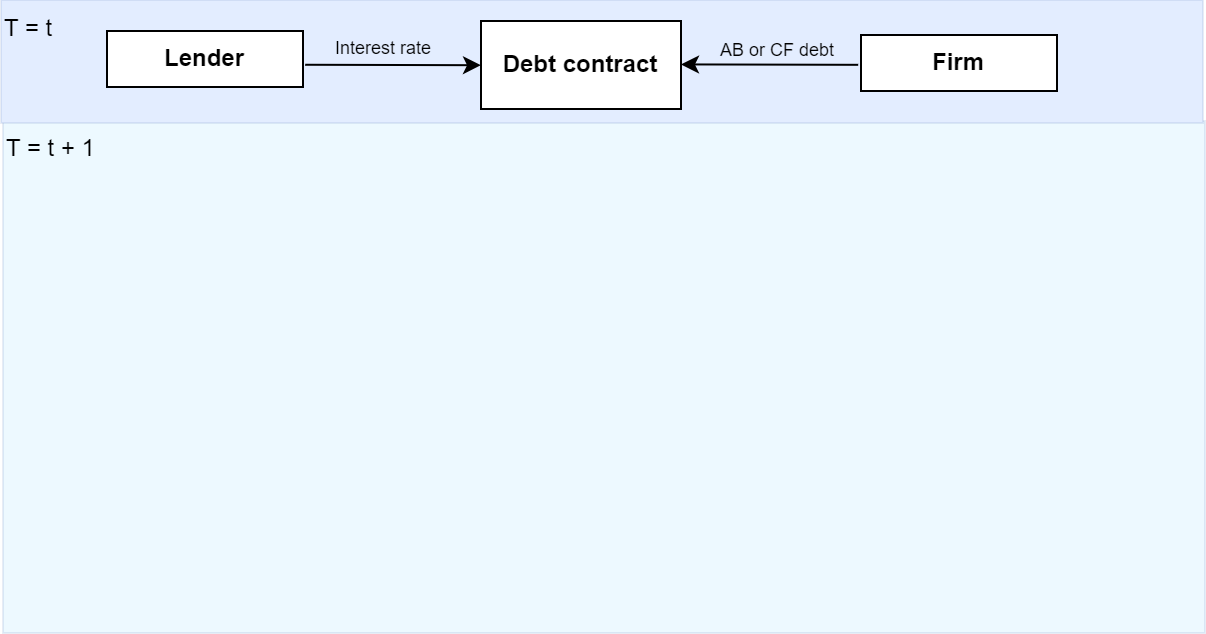
\includegraphics[width=0.95\textwidth]{Plots/min60_t1.png}}
\only<2>{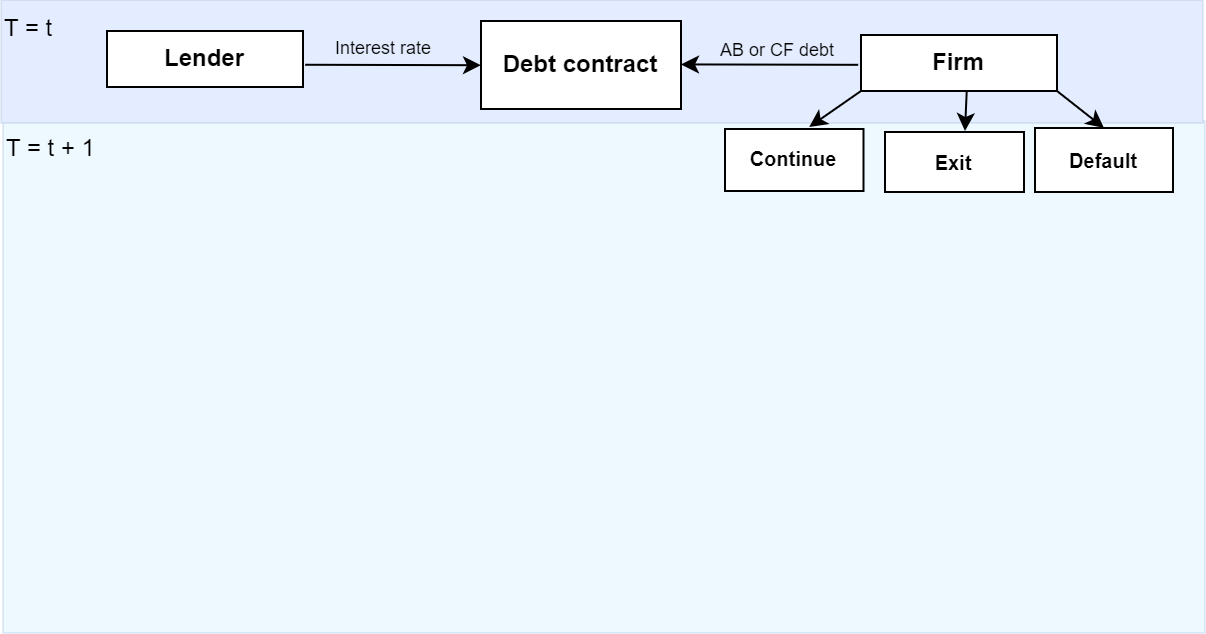
\includegraphics[width=0.95\textwidth]{Plots/min60_t2.png}}
\only<3>{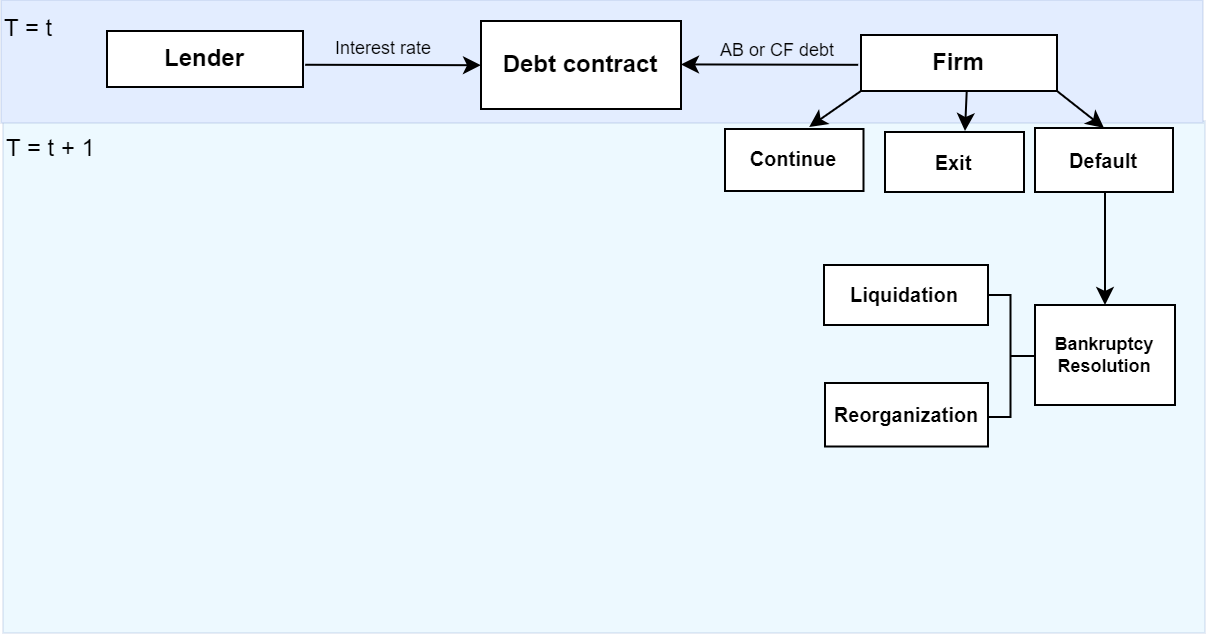
\includegraphics[width=0.95\textwidth]{Plots/min60_t4.png}}
\only<4>{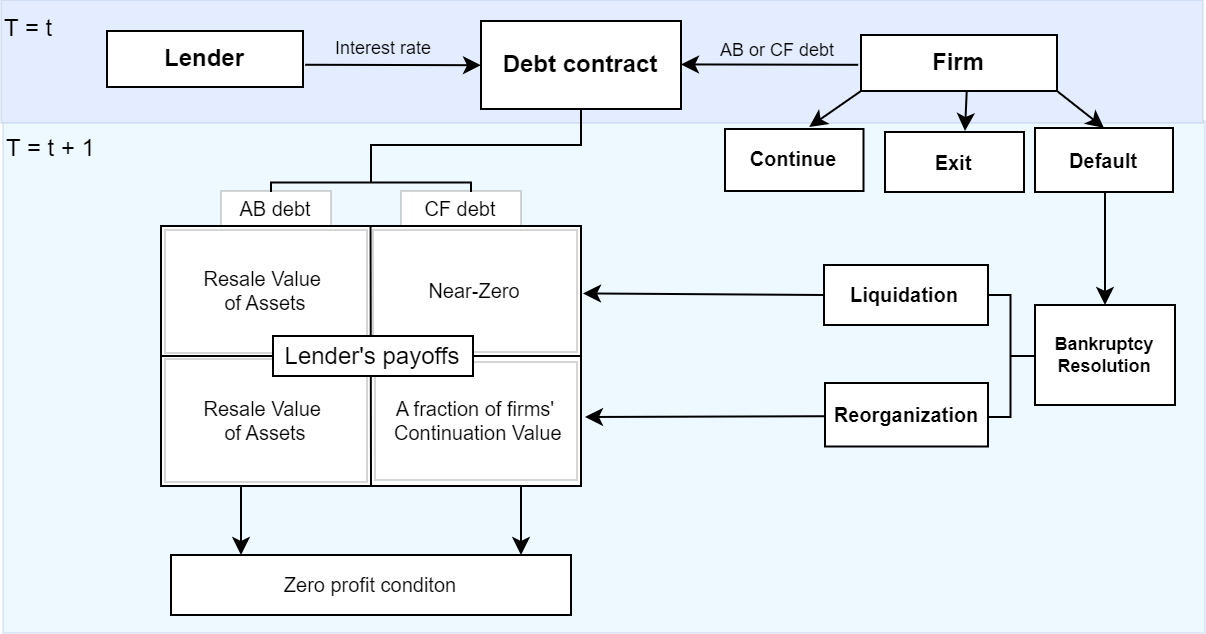
\includegraphics[width=0.95\textwidth]{Plots/min60_t6.png}}
\only<5>{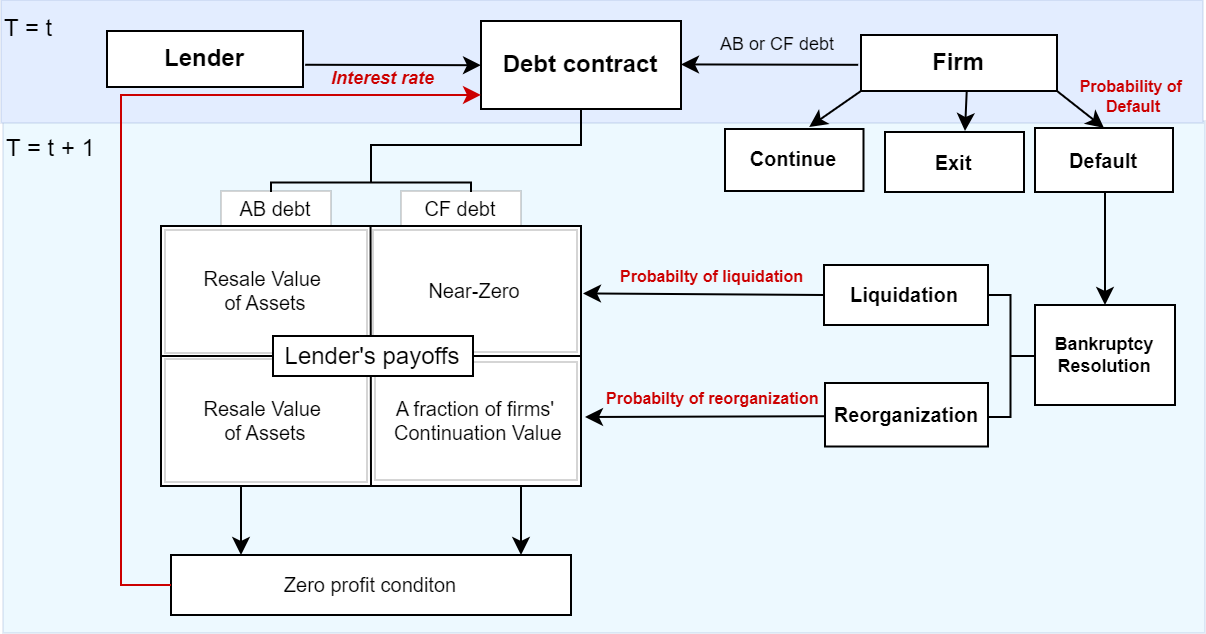
\includegraphics[width=0.95\textwidth]{Plots/min60_t7.png}}

\end{frame}


%------------------------------------------------
\begin{frame}[label=Firms] \frametitle{Production}

Heterogeneous firms: 
\begin{itemize} \small
    \item Capital ($k$), Debt ($b$), Idiosyncratic productivity ($\varepsilon$)
\end{itemize} 
Firm productivity follows an AR(1) process, with \textit{i.i.d.} innovations \normalsize \vspace{3mm}

Produce a homogeneous good, using labor $n$ and capital $k$,
$$ y = \varepsilon k^{\alpha}n^{\nu}, \ \ \ \ \alpha,\nu \in (0,1),  \ \nu + \alpha < 1 $$
Every firm $(k,\varepsilon)$ faces the same optimization w.r.t. labor:
$$ \pi(k,\varepsilon) = \max_{n} \ \  \varepsilon k^{\alpha}n^{\nu} - wn - c$$ 
Fixed cost of production: $c$

\end{frame}


%------------------------------------------------
\begin{frame}[label=Firmvalues] \frametitle{Firm Values}

Incumbents may decide to exit, default or continue production: 
\begin{equation*} \label{eq:default decision}
    V_0(k,b,\varepsilon) = \max \{V_{def}, \  V_{exit}(k,b,\varepsilon),  \ V_{cont}(k,b,\varepsilon) \}
\end{equation*}
Default has zero value
$$ V_{def} = 0 $$ 
Voluntarily exit allows to keep the cash on hand, $x$ 
 $$    V_{exit}(k, b, \varepsilon) =  \underbrace{\pi(k,\varepsilon) + (1-\delta)k - b}_{\textcolor{red}{\text{Cash on Hand}}}  = x $$
Exiting firms are balanced by a mass $M$ of potential entrants \hfill \hyperlink{Entrants}{\beamergotobutton{Entry decision}}
\end{frame}

%------------------------------------------------
\begin{frame}[label= ContFirms] \frametitle{Continuing Firms \hfill\hyperlink{Qfull}{\beamergotobutton{Back to q}}}

Continuing firms maximize the discounted sum of dividends $(d)$ choosing
\begin{itemize} \small
    \item Capital $k'$; One-period debt $b'$; CF-based to total debt, $\tau' \in [0,1]$
\end{itemize} \normalsize


\begin{equation*} \label{eq:V_cont}
    V_{cont}(x,\varepsilon) = \max_{k',b', \tau'} \left( d + q_f \E_{\varepsilon'|\varepsilon} V_0(k',b', \varepsilon') \right)
\end{equation*}
subject to: 
$$ d = x - k' +  \underbrace{q(k',b',\tau', \varepsilon)}_{\textcolor{red}{\text{Inverse interest rate}}} b' $$
\begin{equation*} \label{eq:budget}
x' = \pi(k',\varepsilon')+(1-\delta)k'-b' \hspace{5mm} \text{and} \hspace{5mm} d \geq 0
\end{equation*} 

\begin{itemize} \small
    \item where $q(a',\varepsilon) $ is the inverse gross interest rate, and $a' = (k',b',\tau')$
\end{itemize} \normalsize
Continuing firms: no equity finance, $d \geq 0$
 
\end{frame}



%------------------------------------------------
\begin{frame}[label=slide2] \frametitle{Model Outline: Financial Intermediation}
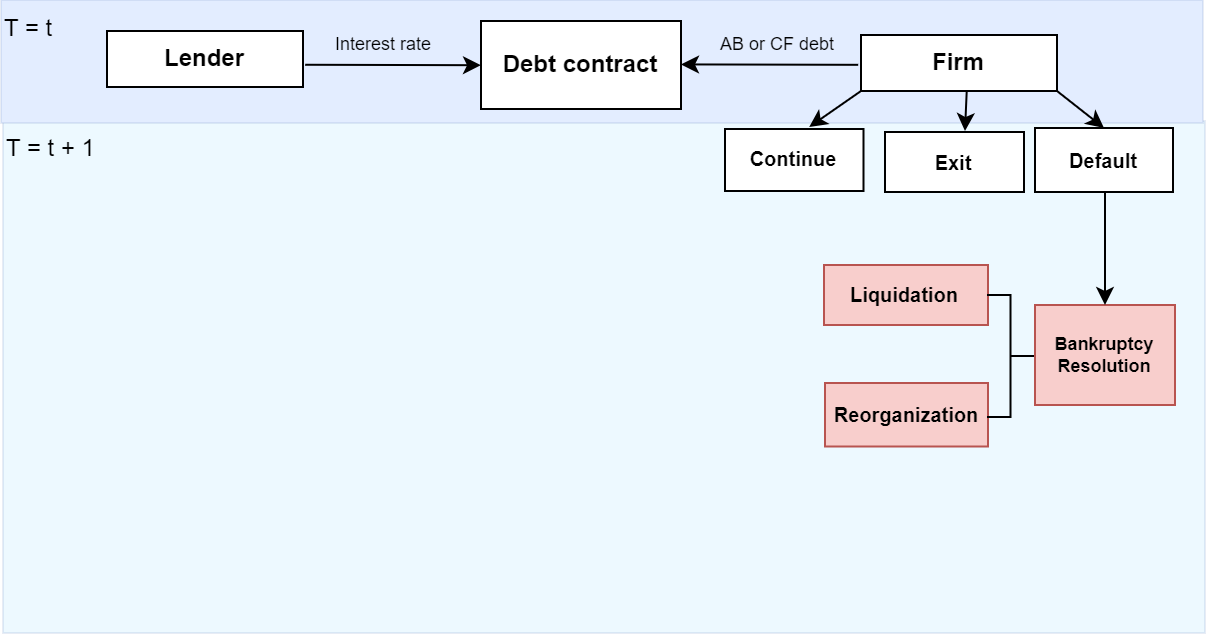
\includegraphics[width=0.95\textwidth]{Plots/red_tmin2.png}
\end{frame}

%------------------------------------------------
\begin{frame}[label=LiqReorg] \frametitle{Default Resolution}

In default: liquidation or reorganization \hfill \hyperlink{Default}{\beamergotobutton{Default Probability }} \vspace{5mm}

Liquidation \textit{(Chapter 7)}:
\begin{itemize} \small
    \item \textbf{Firm exits} and capital stock is resold at a discount, $\phi_a(1-\delta)k$
    \item Liquidation revenues are split between the lender and the household
\end{itemize} \normalsize \vspace{7mm}

Reorganization \textit{(Chapter 11)}:
\begin{itemize} \small
    \item Debt contract is renegotiated at a variable $\phi_c V_{cont}(x,\varepsilon)$ and fixed cost $\zeta$
    \item \textbf{Firm continues,} outstanding debt is replaced by a transfer from the household
\end{itemize} \normalsize   

\end{frame}

%------------------------------------------------
\begin{frame}[label=LiqReorg2] \frametitle{Liquidation Probability}

Bankruptcy courts maximize the \textit{joint value} retained after bankruptcy,
\begin{equation*} \label{eq:liquidation decision}
    \max \{ \underbrace{\phi_a (1-\delta) k}_{\textcolor{red}{\text{Value in Liquidation}}}   ; \ \underbrace{(1-\phi_c) V_{cont}(x,\varepsilon)- \zeta}_{\textcolor{red}{\text{Value in Reorganization}}}   \} 
\end{equation*}


Ex-ante, conditional probability of liquidation in default: 
\begin{equation*} \label{eq:liquidation probability}
    \gamma(k', b', \varepsilon) = Pr(\phi_a (1-\delta) k' \ \geq \ (1-\phi_c) V_{cont}(x',\varepsilon') - \zeta | \chi_d = 1)
\end{equation*}  
\small where $\chi_d$ is a dummy indicating default \normalsize \vspace{5mm} \\
\textbf{Fixed costs} of reorganization, $\zeta$ decreasing liquidation prob. across firm size     \hfill \hyperlink{liqprob}{\beamergotobutton{Data}}

\end{frame}

%------------------------------------------------
\begin{frame}[label = FCreorg] \frametitle{Fixed Costs of Reorganization \hfill \hyperlink{motivation2}{\beamergotobutton{Back to Motivation}}}



Reorganization: lengthy negotiation between debtors and creditors 
\begin{itemize} \small 
    \item Large legal, administrative and time (direct and indirect)  cost
    \item Often involves the costs of replacing original management
\end{itemize} \normalsize \vspace{10mm}  

\textbf{Fixed cost} of reorganization - \footnotesize \textit{Wang, 2022,  Bris et al. 2006, LoPucki and Doherty, 2011} 
\begin{itemize} \small 
    \item Smaller firms face higher reorganization costs per dollar of assets
    \item Smaller firms take longer to reorganize per dollar of assets \hfill \hyperlink{daysin111}{\beamergotobutton{Details}}
\end{itemize} \normalsize \vspace{3mm}



\end{frame}


%------------------------------------------------
\begin{frame}[label = payoffs]
\frametitle{The Lender's Recovery}

\only<1->{
\begin{table}[h!]
\centering
\resizebox{0.57\textwidth}{!}{% 0.75 times the text width
\begin{tabular}{l|cc}
& Asset-based debt & CF-based debt  \\  
  \midrule
Liquidation & $ \only<1>{\textcolor{red}{\phi_a (1-\delta)k}} $  $ \only<2->{\phi_a (1-\delta)k} $ &  \only<3>{\textcolor{red}{$ \kappa\phi_a (1-\delta) k$}} \only<4>{$ \kappa\phi_a (1-\delta) k$} \\ 
Reorganization & \only<4->{\textcolor{red}{ $\phi_a (1-\delta) k $}} & \only<2>{\textcolor{red}{$\theta V_{cont}(x, \varepsilon)$}} \only<3->{$\theta V_{cont}(x, \varepsilon)$} \\ 
\bottomrule
\end{tabular}
}
\label{tab:shares}
\end{table}}

\only<1-2>{ 
Recovery of asset-based debt under liquidation: 
\begin{itemize} \small
    \item Backed by physical collateral, recovers:  $ \phi_a (1-\delta) k$
\end{itemize} \normalsize
}

\only<2>{
Recovery of CF-based debt under reorganization:  
\begin{itemize} \small
    \item  Debt renegotiation outcome: $\theta V_{cont}(x,e)$ \qquad - \footnotesize {Corbae and D'Erasmo, 2021}
\end{itemize} \normalsize
}

\only<3-4>{
Recovery of CF-based debt under liquidation: \hfill \hyperlink{payoffs_det}{\beamergotobutton{Details}}
\begin{itemize} \small
    \item Not backed by physical collateral
    \item Near-zero recovery: $\kappa \phi_a (1-\delta) k$, where  $ \kappa \in (0,1)$ \qquad \footnotesize - Bris et al. (2006) 
\end{itemize} \normalsize
}

\bigskip
      
\only<4>{
Recovery of asset-based debt under reorganization: 
\begin{itemize} \small
    \item Creditor is protected by the 'best interest of creditor test'  - \textit{U.S.C. §1129}
    \item Recovery is \textit{expected} to match the resale value of assets: $\phi_a (1-\delta) k$
\end{itemize} \normalsize }

\end{frame}

%------------------------------------------------
\begin{frame}[label=Lpayoff] \frametitle{The Lender's In-Default Payoffs \hfill\hyperlink{HH_T}{\beamergotobutton{Household Payoffs}} }

\begin{table}[h!]
\centering
\resizebox{0.55\textwidth}{!}{
\begin{tabular}{l|cc}
& Asset-based debt & CF-based debt  \\  
\midrule
Liquidation & $\phi_a (1-\delta) k$ & $\kappa\phi_a (1-\delta) k$ \\ 
Reorganization & $\phi_a (1-\delta) k$ & $\theta V_{cont}(x, \varepsilon)$ \\ 
\bottomrule
\end{tabular}
}
\label{tab:shares}
\end{table}

Under liquidation, the lender recovers 
$$   \Pi_{l}(a) =  \min \{b, \ \ (1-\tau) \underbrace{\phi_a (1-\delta) k}_{\textcolor{red}{\text{AB, Liq}}} + \tau \underbrace{\kappa \phi_a  (1-\delta) k}_{\textcolor{red}{\text{CF, Liq}}} \} $$
\begin{itemize} \small
    \item The remainder is retained by the household
\end{itemize} \normalsize
Under reorganization, the lender negotiates the transfer: 
$$ \Pi_{r}(a,\varepsilon) = \min \{b, \ \  (1-\tau) \underbrace{\phi_a (1-\delta) k}_{\textcolor{red}{\text{AB, Reorg}}} +\tau \underbrace{\theta V_{cont} (x, \varepsilon)}_{\textcolor{red}{\text{CF, Reorg}}} \} $$ 

 
\end{frame}



%------------------------------------------------
\begin{frame}[label=slide2] \frametitle{Model Outline: Financial Intermediation}

\only<1>{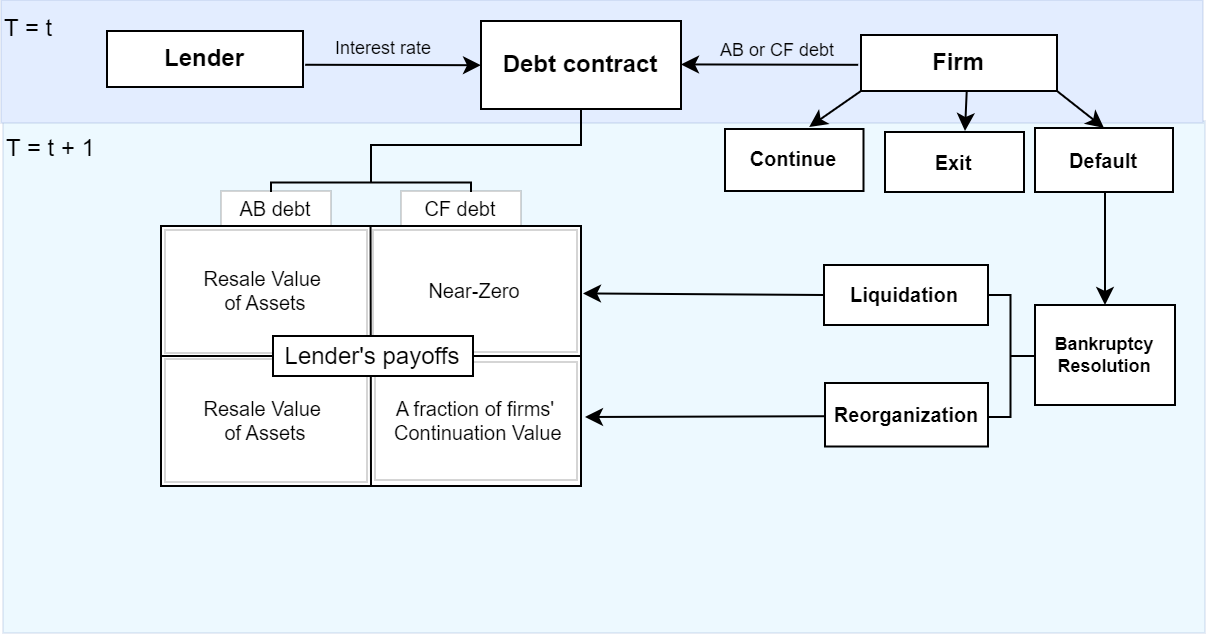
\includegraphics[width=0.95\textwidth]{Plots/min60_t5.png}}
\only<2>{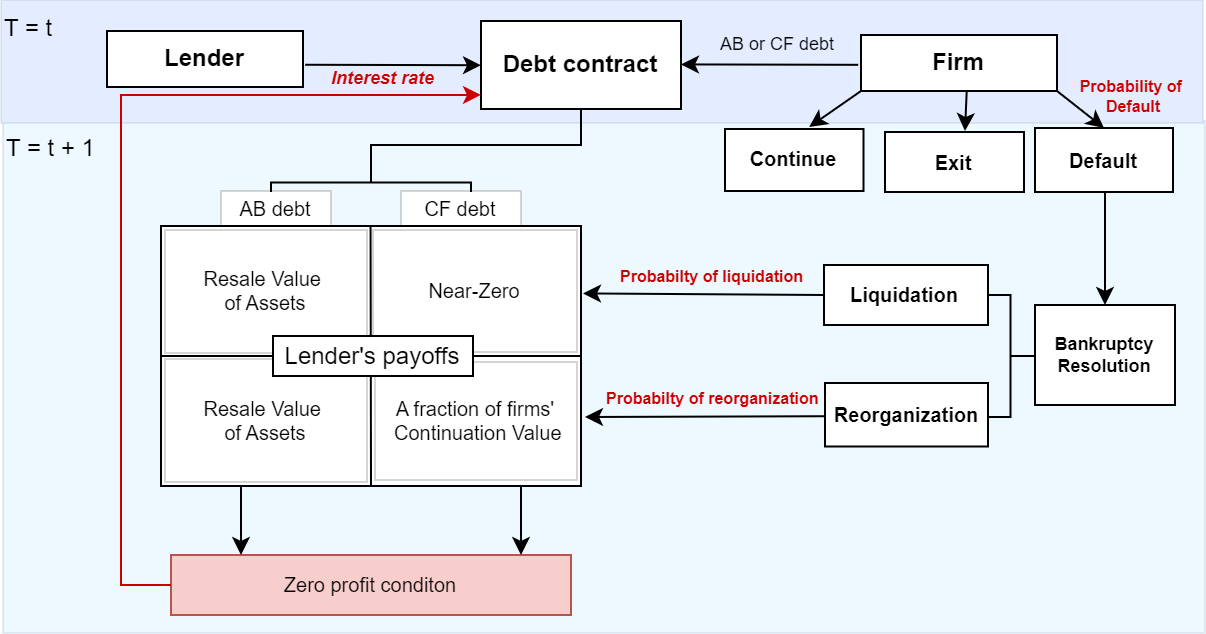
\includegraphics[width=0.95\textwidth]{Plots/red_tmin.png}}


\textbf{}\end{frame}



%------------------------------------------------
\begin{frame}[label=Qfull] \frametitle{The Inverse Interest Rate  \hfill \hyperlink{mechanism}{\beamergotobutton{Model Mechanism}} \hyperlink{ContFirms}{\beamergotobutton{Firm optimization}}}

The lender considers: \small 
\begin{itemize}\setlength\itemsep{0em} 
    \item Probability of default, $P_D(a', \varepsilon)$
    \item Probability of liquidation in default $\gamma(k',b', \varepsilon)$
    \item Expected payoffs under liquidation and reorganization,  $\Pi_{l}(a')$, $\Pi_{r}(a', \varepsilon)$
\end{itemize} \normalsize

Inverse interest rate ($q$) defined by the zero profit condition:
\begin{equation*} \label{eq:q}
    \begin{split}
        & q(a', \varepsilon)b' = q_0 [ \left(1-P_D(a', \varepsilon)\right)b' +  \\
        & \qquad \qquad \underbrace{P_D(a', \varepsilon)}_{\textcolor{red}{\text{Pr(Default)}}} \underbrace{\gamma(a', \varepsilon)}_{\textcolor{red}{\text{\quad Pr(Liq.) \quad }}} \underbrace{\Pi_{l}(a')}_{\textcolor{red}{\text{Recovery Liq. }}} + \\  
        & \qquad  \qquad \underbrace{P_D(a', \varepsilon)}_{\textcolor{red}{\text{Pr(Default)}}}  (\underbrace{1-\gamma(a', \varepsilon)}_{\textcolor{red}{\text{Pr(Reorg.) }}})\ E_{\varepsilon' | \varepsilon} [ \underbrace{\Pi_{r}(a', \varepsilon')}_{\textcolor{red}{\text{Recovery Reorg. }}} |\chi_r = 1 ] \} ]
    \end{split}
\end{equation*}

Continuing firms choose $(k',b',\tau')$, to maximize $V_{cont}(x,\varepsilon)$ s.t. $q(k',b',\tau', \varepsilon)$ 

\end{frame}


\section{Calibration and Model Fit}

%------------------------------------------------
\begin{frame}[label=Calibration] \frametitle{External Calibration}

\begin{table}[h!]
    \centering
    \resizebox{0.8\textwidth}{!}{
    \renewcommand{\arraystretch}{0.85}  
    \begin{tabular}{c|c|c|c}
    \multicolumn{4}{l}{\textbf{Externally Calibrated Parameters}} \\ 
    \toprule
    Parameter & Description & Value & Source/Note \\
    \midrule
    $\beta$ & Discount Rate & 0.96 & \textit{Standard} \\
    $\alpha$ & Capital Share & 0.25 & \textit{Standard} \\
    $\nu$ & Labour Share & 0.5 & \textit{Standard} \\
    $\delta$ & Depreciation rate & 0.065 & Khan and Thomas (2013) \\
    $\rho$ & Productivity Shock Persistence & 0.969 & Di Nola et al. (2023) \\
    $\sigma_{\varepsilon}$ & Productivity Shock SD & 0.146 & Di Nola et al. (2023) \\
    $\varepsilon_0$ & Average Productivity & 1 & Di Nola et al. (2023) \\
    $\phi_a$ & Resale value of assets & 0.4 & Kermani et al. (2020) \\
    $\kappa$ & Unsecured discount & 0.1 & \textcolor{gray}{Bris et al. (2006)} \\
    \bottomrule
    \end{tabular}
    }
    \label{tab:external calib}
\end{table}
Based on standard values in the literature and empirical estimations 


\end{frame}


\begin{frame}{Internal Calibration and Model Fit}

Data: US non-financial firms, 2010-2024  \hfill \hyperlink{targets}{\beamergotobutton{Details}}
\begin{itemize} \small
    \item Firm- and Debt-level data: Compustat connected to Capital IQ
    \item Bankruptcy resolution: Federal Judicial Center, Integrated Database (IDB)
\end{itemize}  


\small
\begin{table}[h!]
\centering
\renewcommand{\arraystretch}{0.85}

\begin{minipage}{0.51\textwidth}
\centering
\resizebox{\textwidth}{!}{
\begin{tabular}{c|l|c}
\multicolumn{3}{l}{\textbf{Internally Calibrated Parameters}} \\
\toprule
Parameter & Description & Value \\
\midrule
$c_e$ & Entry cost & 654.3  \\
$\phi_c$ & Variable cost of reorganization & 0.197 \\
$\zeta$ & Fixed costs of reorganization & 2753 \\
$\theta$ & Lender's payoff under reorganization & 0.361 \\
$P_x$ & Exogenous default probability & 0.029 \\
$c$ & Fixed costs of operation & 42.03 \\
\bottomrule
\end{tabular}
}
\label{tab:internal_calib}
\end{minipage}
\hfill
\begin{minipage}{0.47\textwidth}
\centering
\resizebox{\textwidth}{!}{
\begin{tabular}{c|c|c}
\multicolumn{3}{l}{\textbf{Targeted moments}} \\
\toprule
SS value & Target value & Model value \\
\midrule
Wage & 1 & 1 \\
Liquidation prob. & 0.58 & 0.56 \\ 
Debt to Collateral & 0.52 & 0.50 \\ 
Interest rate & 5.36 & 5.30 \\ 
CF-reliance & 0.51 & 0.53 \\ 
CF-based to total debt & 0.82 & 0.82 \\ 
\bottomrule
\end{tabular}
}
\label{tab:targets}
\end{minipage}

\end{table}
\normalsize

\begin{itemize} \small
    \item Targeted moments computed by mapping Compustat means onto IDB size distribution \normalsize
\end{itemize}  
    
\end{frame}


%------------------------------------------------
\begin{frame}[label=3] \frametitle{Model Fit - Untargeted Moments}


Classification: small and large firms  \small
\begin{itemize}
    \item Based on borrowing, approx. 60\% are small
\end{itemize} \normalsize 
Data moments and corresponding \textcolor{red}{Model Values}

\small
\begin{table}[h!]
    \centering
    \renewcommand{\arraystretch}{0.9}
        \begin{tabular}{c|c|c}
        \multicolumn{3}{l}{\textbf{Untargeted moments}} \\ 
        \toprule
         Data - \textcolor{red}{Model} & Small firms &  Large firms  \\
         \midrule
         Liquidation Probability  & 0.84 - \textcolor{red}{0.85}  & 0.20 - \textcolor{red}{0.14}  \\
         Debt to Collateral & 0.44 - \textcolor{red}{0.45}  & 0.59 - \textcolor{red}{0.57}  \\
         Interest Rate (\%) & 5.89 - \textcolor{red}{5.63}  & 4.63 - \textcolor{red}{4.89}  \\
         Reliance on CF-debt  &  0.51 - \textcolor{red}{0.24}  &  0.53 - \textcolor{red}{0.97}  \\
         CF-based to total debt & 0.34 - \textcolor{red}{0.30}  & 0.83 - \textcolor{red}{0.87}  \\
        \bottomrule
        \end{tabular}
    \label{tab:external calib} 
\end{table}
\normalsize

\end{frame}

\section{Model Results}


%------------------------------------------------
\begin{frame}[label = Pexp]  \frametitle{Main Results}

\textbf{Model experiment:} cutting the fixed reorganization cost to half
\begin{itemize} \small
    \item Average liquidation probability falls from $\sim 56\%$ to $\sim 39\%$
\end{itemize} 

\small
\begin{table}[h!]
    \centering
    \renewcommand{\arraystretch}{0.85}
    \begin{tabular}{l|c|c}
    \multicolumn{3}{l}{\textbf{Steady State Moments}} \\ 
    \toprule
     Baseline - \textcolor{red}{Reform} & Small Firms & Large Firms \\
    \midrule
    Pr. Liquidation & 0.86 - \textcolor{red}{0.63} & 0.14 - \textcolor{red}{0.03} \\ 
    Debt/Collateral & 0.45 - \textcolor{red}{0.48} & 0.57 - \textcolor{red}{0.57} \\ 
    Interest Rate & 5.63 - \textcolor{red}{5.23} & 4.89 - \textcolor{red}{4.63} \\  
    CF Reliance & 0.24 - \textcolor{red}{0.43} & 0.97 - \textcolor{red}{0.99} \\ 
    CF-based to Total Debt & 0.30 - \textcolor{red}{0.72} & 0.87 - \textcolor{red}{0.92} \\ 
    \bottomrule
    \end{tabular}
    \label{tab:SSvalues_compact}
\end{table} \normalsize

Financing gap narrows
\begin{itemize} \small
    \item Small firms: lower liquidation risk $\rightarrow$ higher borrowing at lower rates
    \item Large firms: already low liquidation risk $\rightarrow$ limited impact
\end{itemize} 

\end{frame}




%------------------------------------------------
\begin{frame}[label = Pexp]  \frametitle{Main Results}

Aggregate effects of the reform

\small
\begin{table}[h!]
    \centering
    \renewcommand{\arraystretch}{0.85}
    \begin{tabular}{l|c|c|>{\columncolor{blue!10}}c}
    \multicolumn{4}{l}{\textbf{Steady State Moments}} \\ 
    \toprule
     & \textbf{Baseline} & \textbf{Reform} & \textbf{\% Change} \\ 
     \midrule
     Number of Firms & 10.00 & 10.71 & +7.10\% \\ 
     Mean Employees & 999 & 933 & -6.61\% \\
     Capital Intensity (K/L) & 3.42 & 3.52 & +2.92\% \\ 
     Productivity (Y/L) & 2.00 & 2.035 & +1.75\% \\
    \bottomrule
    \end{tabular}
  \label{tab:ss_moments}
\end{table}
\normalsize

Sizable productivity gains
\begin{itemize} \small
    \item Cheaper access to external finance $ \rightarrow $ higher capital intensity
    \item Higher ex-ante value of entering $\rightarrow$ higher firm mass
    \item Aggregate productivity improves by $1.75\%$
\end{itemize} \normalsize


\end{frame}



%------------------------------------------------
\begin{frame}[label=Decomp_main] \frametitle{Decomposition of Productivity Gains  \hfill  \hyperlink{decompA}{\beamergotobutton{Derivations}}}

Output per worker increases by \textbf{1.75\%} after the reform. \vspace{3mm} \\

Can be decomposed into,
\begin{itemize} \small
    \item \textbf{Capital deepening:} driven by changes in the capital stock
    \item \textbf{Mass effect:} driven by the number of operating firms  
    \item \textbf{Composition effect:} driven by the distribution of firms across productivity states 
    \item \textbf{Policy residual:} driven by changes in firms’ individual capital and financing policies 
\end{itemize} \normalsize


\[
\Delta\log\frac{Y}{N}
= \underbrace{\frac{\alpha}{1-\alpha}\,\Delta\log\frac{K}{Y}}_{\text{Capital Deepening}}
+ \frac{1}{1-\alpha}\Big[
\underbrace{(1-s)\Delta\log M}_{\text{Mass Effect}} +  
\underbrace{(1-s)\Delta\log C}_{\text{Composition Effect}} + 
\underbrace{\Delta\log\Omega}_{\text{Policy Residual}}\Big].
\] 

\small where $s$ is the Lucas' span-of-control parameter



\end{frame}


%------------------------------------------------
\begin{frame}[label=decomp3] \frametitle{Decomposition Results: Drivers of Productivity Gains}

\small
\begin{table}[h!]
\centering
\renewcommand{\arraystretch}{0.9}
\begin{tabular}{lcc}
\toprule
 & Log-point Change & Share of Total \\
\midrule
Output per worker, $Y/L$    & 1.735 & 1.00 \\
\midrule
Capital Deepening ($K/Y$)   & 0.295 & 0.17 \\
Mass Effect ($M$)           & 2.802 & 1.61 \\
Composition Effect ($C$)    & -1.672 & -0.96 \\
Policy Residual ($\Omega$)  & 0.311 & 0.18 \\
\bottomrule
\end{tabular}
\end{table}
\normalsize

\begin{itemize} \small
    \item \textbf{Capital deepening:} better access to debt finance
    \item \textbf{Mass effect:} higher number of active firms raise productivity 
    \item \textbf{Composition effect:} leftward shift in the firm distribution reduces productivity 
    \item \textbf{Policy residual:} firm policies change relatively little 
\end{itemize}



\end{frame}



%------------------------------------------------
\begin{frame}[label=distplot] \frametitle{Decomposition of Productivity Gains \hfill  \hfill \hyperlink{Entrants}{\beamergotobutton{Entry Decision}}}

Comparison of capital allocation across \textbf{Perfect Credit}, \textcolor{blue}{Baseline}, and \textcolor{red}{Reform}

\begin{figure}[h!]
    \centering
    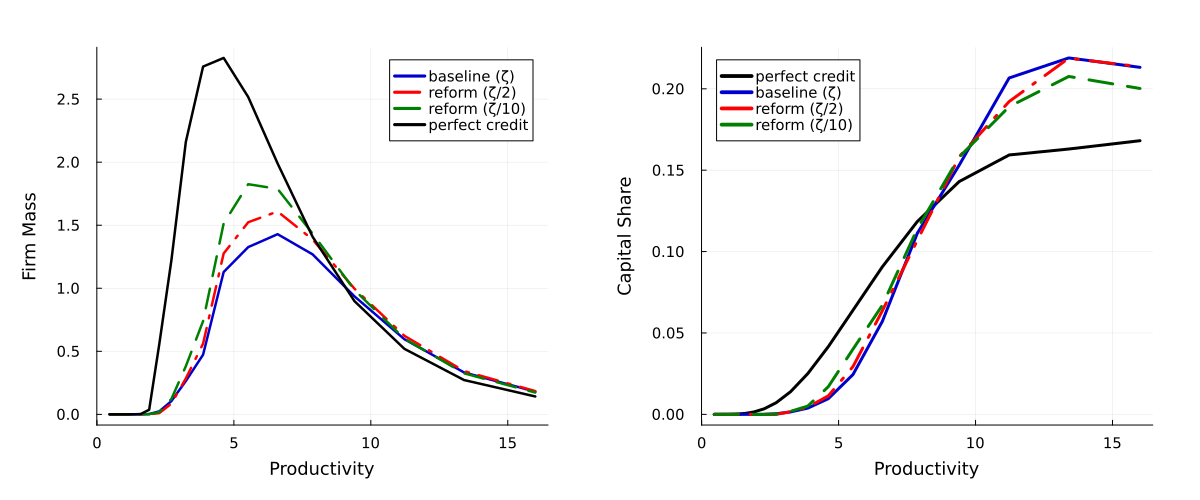
\includegraphics[width=0.85\textwidth]{Plots/Combined4runs2.png}
    \label{fig:GamPol}
\end{figure} \vspace{-2mm}

\begin{itemize}\small
    \item Credit frictions allow highly productive (large) firms to capture an excessive market share
    \item Reducing credit frictions allows more low- and medium productivity firms to operate
\end{itemize}

\end{frame}


%------------------------------------------------
\begin{frame}[label=Aggeffects] \frametitle{The Effects of Reorganization Costs - Alternative Models \hfill  \hyperlink{liqrisk}{\beamergotobutton{Intuition}}}

Cutting the fixed reorganization cost in alternative model setups

\small
\begin{table}[H]
    \centering
    \renewcommand{\arraystretch}{0.85}
    \begin{tabular}{lccc}
    & \textbf{Baseline Calib.} & \textbf{Only asset-based} & \textbf{Only CF-based} \\    
    \toprule
    \rowcolor{blue!10} Pr. Liquidation & -17.41 pp & -18.32 pp & -21.69 pp \\  
    \rowcolor{blue!10} Productivity (Y/L) & 1.75\% & 0\% & 2.40\% \vspace{2mm} \\  

    Debt/Collateral & 2.57 pp & -0.87 pp & 5.82 pp \\  
    Interest rate & -0.34 pp & -0.03 pp & -0.71 pp \\  
    Number of firms & 7.1\% & 1.14\% & 20.91\% \\  
    Mean employees & -6.61\% & -1.13\% & -17.29\% \\  
    \bottomrule
    \end{tabular}
    \label{tab:percentage_changes}
\end{table}
\normalsize

\begin{itemize} 
    \item Only Asset-based debt is available $\rightarrow$ negligible effects
    \item Only CF-based debt is available $\rightarrow$ over-estimated effects
\end{itemize} 


\end{frame}


\section{Designing Bankruptcy Frameworks}


%------------------------------------------------
\begin{frame}[label=EUandUS]  \frametitle{Bankruptcy Reforms in the EU and U.S. \hfill \hyperlink{sbra_emp}{\beamergotobutton{SBRA Empirical}} \hyperlink{SBRA}{\beamergotobutton{SBRA Model Effects}}  }

Recent efforts to streamline reorganization
\begin{itemize} \small
    \item U.S.: Small Business Reorganization Act \hspace{11mm }\textit{- SBRA, February 2020} 
    \item EU: Preventive Restructuring Directive \hspace{12.32mm} \textit{- Directive (EU) 2019/1023}
    \item Spain: Reform of the Insolvency Act \hspace{16mm} \textit{- Law 16/2022}

\end{itemize} \normalsize 
\textbf{EU}: Mandatory early-warning tools; \quad \textbf{U.S.}: Targeted support for small firms  \vspace{5mm} \\

Several provisions aim to facilitate reorganization:
\begin{itemize} \small
    \item Simplified procedures and reduced disclosure requirements \hfill \textit{EU \& U.S.}
    \item More flexible plan confirmation, cramdown of dissenting creditors \hfill \textit{EU \& U.S.}
    \item Appoints a `Subchapter V trustee' to facilitate negotiations \hfill \textit{U.S.} 
\end{itemize} \normalsize

\end{frame}



%------------------------------------------------
\begin{frame}[label=Framework] \frametitle{Efficient Policy Design}

Policy experiments
\footnotesize
\begin{table}[H]
    \centering
    \renewcommand{\arraystretch}{0.9}
    \begin{tabular}{lc|c}
    \toprule
    \textbf{Policy reform} & \textbf{$\Delta$ Productivity (Y/L)} & \textbf{Parameter changes} \\
    \midrule
    Universal policy & +0.93\% & $0.75*\zeta$ \\
    Targeted to small firms & +0.81\% & $0.75*\zeta_{\text{small}}$ \\
    Reduced creditor control & -0.54\% & $ 0.75*(\zeta,\theta$) \\
    \bottomrule
    \end{tabular}
    \label{tab:percentage_changes2}
\end{table}
\normalsize


Size-based reforms targeting small and middle-market firms are effective
\begin{itemize}\small
    \item Spain, Book III TRLC: dedicated, simplified insolvency procedure for microenterprises
\end{itemize}
Weaker creditor rights can erode the gains from streamlining reorganization

\end{frame}




%------------------------------------------------
\begin{frame}[label=3] \frametitle{Conclusions}

Most of corporate debt is backed by future cash flows
\begin{itemize} \small
    \item High ex-ante liquidation risk is a major impediment to small firms' access to credit
\end{itemize} \normalsize \vspace{3mm}


Reducing reorganization costs yields sizable productivity gains
\begin{itemize} \small
     \item Lowers liquidation risk, improves access to CF-based debt, promotes firm entry 
     \item A 17pp decline in liquidation risk raises aggregate productivity by 1.75\%
     \item Most gains come from a larger number of operating firms
\end{itemize} \normalsize \vspace{3mm}

Streamlining reorganization improves credit markets and raises productivity
\begin{itemize} \small
     \item Targeted policies are effective, but weakening creditor control erodes the gains
\end{itemize} \normalsize

\end{frame}


\appendix
\section{Appendix}


%------------------------------------------------
\begin{frame}[label = LandM] \frametitle{Cash Flow-Based and Asset-Based Lending \hfill \hyperlink{motivation1}{\beamergotobutton{Back}}}

Asset-based lending:
\begin{itemize} \small
\item Secured against borrowers' physical  assets
\item \textbf{Creditors in-default payoffs}: value of physical collateral
\end{itemize} \normalsize 
Cash flow-based lending:
\begin{itemize} \small
\item No \textit{specific} assets pledged as collateral
\item Secured against the entire corporate entity, or unsecured
\item \textbf{Creditors in-default payoffs}: expected future cash flows
\end{itemize} \normalsize
Lian and Ma (2021): 80\% of US corporate debt is backed by future cash-flows \vspace{3mm}

Different from security: 
\begin{itemize} \small
    \item Secured vs. Unsecured: priority in bankruptcy
        \item Asset vs CF-based: economic determinants of lenders' in-default payoffs
\end{itemize} \normalsize

\end{frame}


%------------------------------------------------
\begin{frame}[label=slide2] \frametitle{Empirical Analysis}

\begin{table}[H]
    \centering
    \renewcommand{\arraystretch}{1.2}
    \resizebox{1\textwidth}{!}{%
    \begin{tabular}{lcccccc}
    \toprule
    & \multicolumn{2}{c}{All contracts} & \multicolumn{2}{c}{CF contracts} & \multicolumn{2}{c}{AB contracts} \\
    \cmidrule(lr){2-3} \cmidrule(lr){4-5} \cmidrule(lr){6-7}
    \textbf{LHS}: Spread & Value & SE & Value & SE & Value & SE \\
    \midrule
    Log of EBITDA & -0.162*** & (0.0102) & -0.106*** & (0.0112) & -0.246*** & (0.0205) \\
    Log of Assets & -0.394*** & (0.0449) & -0.488*** & (0.0538) & -0.264*** & (0.0804) \\
    Pledgeability & -0.526*** & (0.0794) & 0.003 & (0.0950) & -1.132*** & (0.140) \\
    Leverage & 1.712*** & (0.101) & 2.006*** & (0.127) & 1.005*** & (0.170) \\
    Log of Age & -0.142*** & (0.0237) & -0.173*** & (0.0282) & -0.113*** & (0.0407) \\
    \midrule 
    Period, Sector, Rating FE & Yes & & Yes & & Yes & \\
    Observations & 19,256 & & 11,929 & & 7,327 & \\
    R-squared & 0.301 & & 0.419 & & 0.183 & \\
    \bottomrule
    \end{tabular}%
    }
\end{table}


\end{frame}


%------------------------------------------------
\begin{frame}[label = spreads] \frametitle{Spreads Over Size \hfill  \hyperlink{motivation1}{\beamergotobutton{Back  to motivation}}  }

    \begin{figure}
       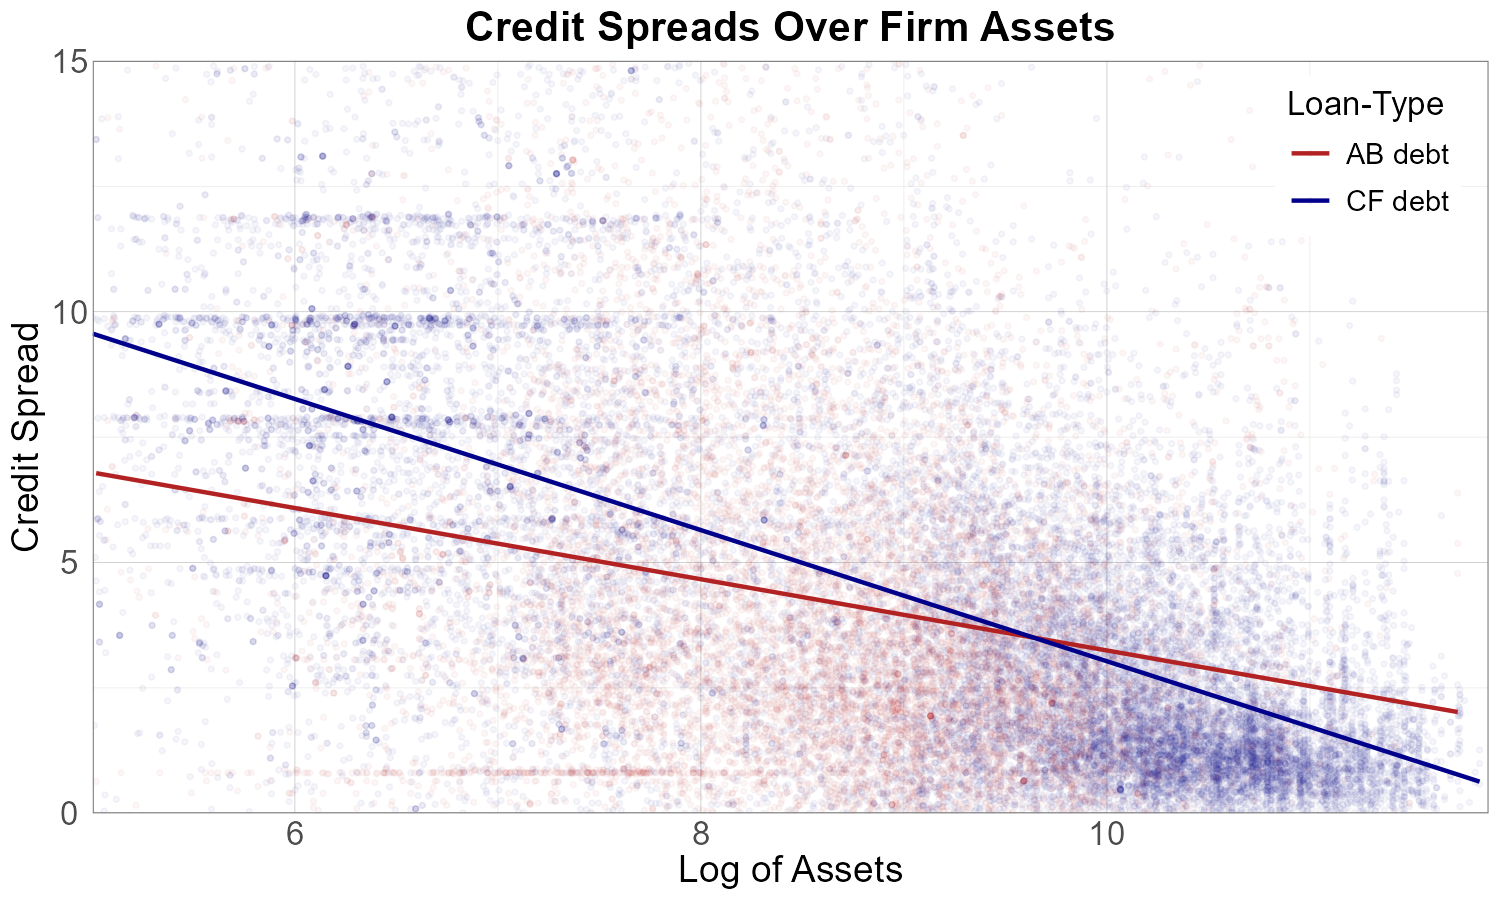
\includegraphics[width=0.85\textwidth]{Plots/spreads.png} 
     \end{figure} \vspace{-4mm}


\end{frame}

%------------------------------------------------
\begin{frame}[label = liqprob] \frametitle{Bankruptcy Resolutions \hfill  \hyperlink{motivation2}{\beamergotobutton{Back  to motivation}} \hyperlink{LiqReorg2}{\beamergotobutton{Back to fixed costs}}}

    \begin{figure}
       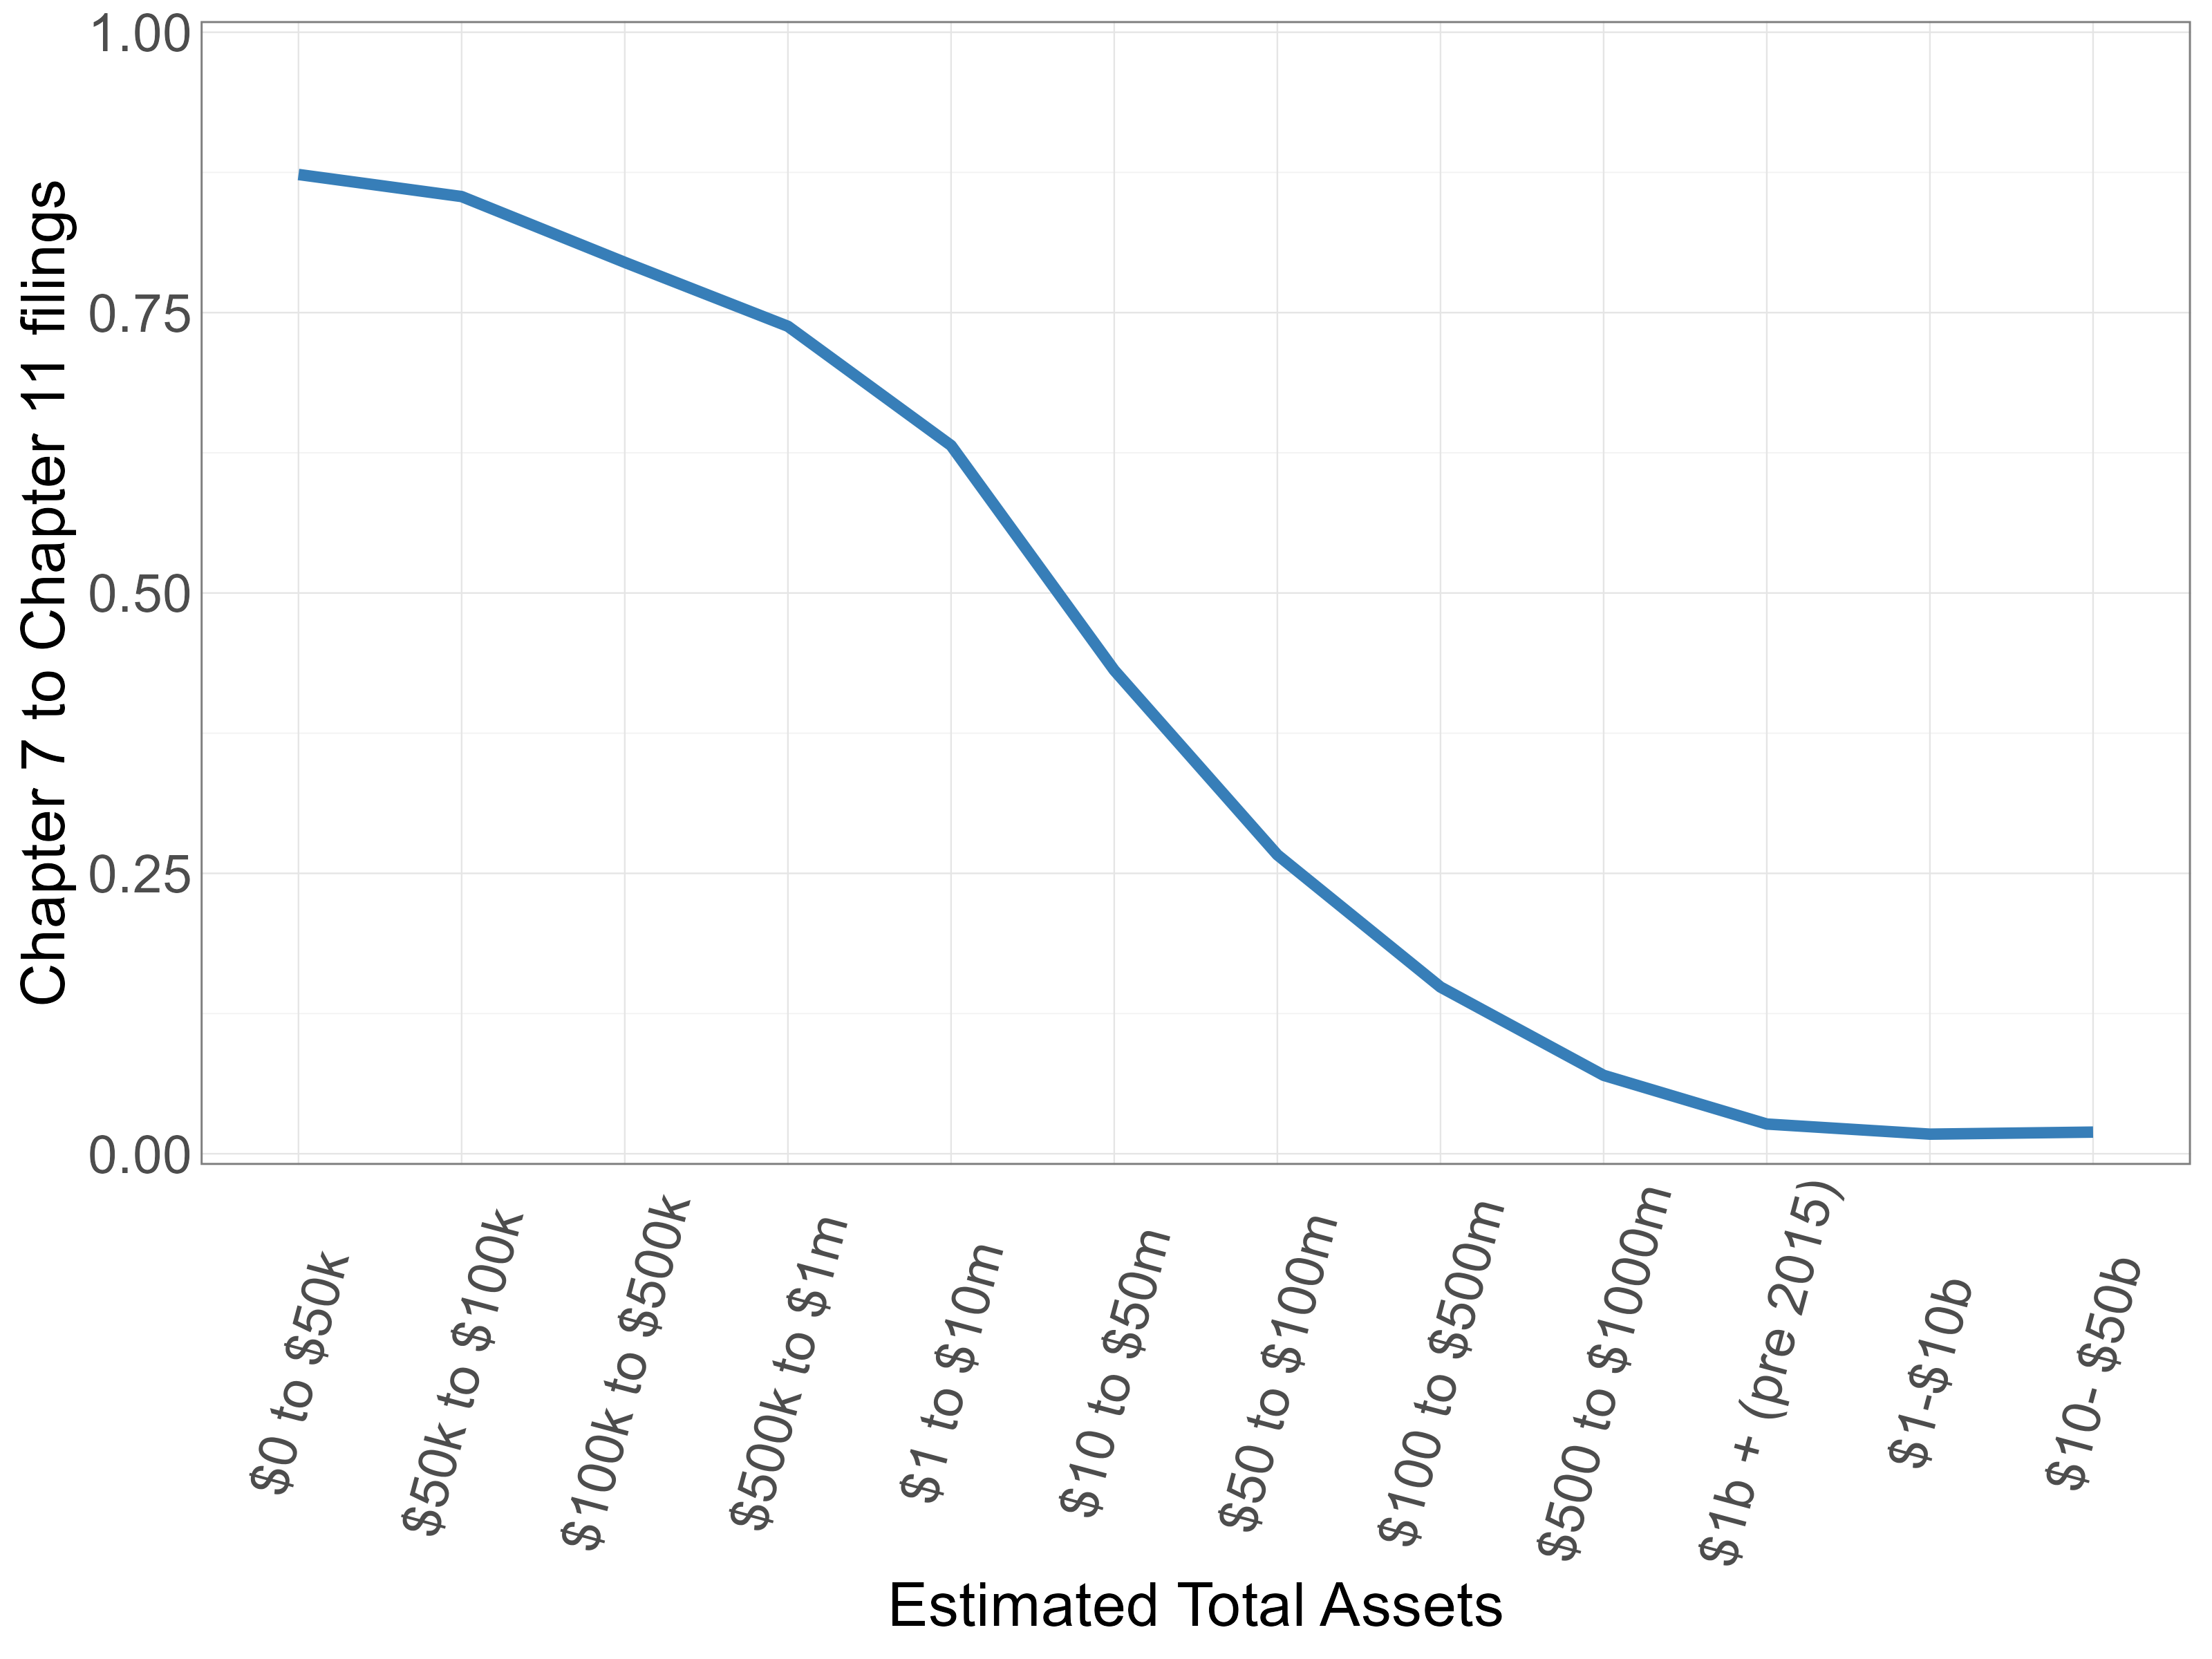
\includegraphics[width=0.7\textwidth]{Plots/liqprob2.png} 
     \end{figure} \vspace{-4mm}


\end{frame}


%------------------------------------------------
\begin{frame}[label = Conversions] \frametitle{Lender's Perspective: Exogenous Risk of Liquidation \hfill  \hyperlink{motivation2}{\beamergotobutton{Back}}}

The debtor is expected to file for bankruptcy
\begin{itemize} \small 
    \item Chapter 7 liquidation or Chapter 11 reorganization
\end{itemize} \normalsize \vspace{6mm} 

Observed Conversions in the US (IDB 2010–2023)
\begin{itemize} \small 
    \item 0.16\% of Chapter 7 cases converted to Chapter 11
\end{itemize} \normalsize  \vspace{6mm}

Legal and practical barriers to reversing liquidation decisions
\begin{itemize} \small
    \item The court is unlikely approve the conversion, if the owners is unwilling to continue 
    \item Lender is often ill-equipped to take over the management of the firm
\end{itemize} \normalsize


\end{frame}



%------------------------------------------------
\begin{frame}[label = payoffs_det] \frametitle{Recovery - Further Details \hfill  \hyperlink{payoffs}{\beamergotobutton{Back}}}

\textbf{Near-zero} recovery of CF-based debt under liquidation: 
\begin{itemize} \small
    \item No physical collateral; recovery is costly and time-consuming
    \item Assets are often tied up in other loans (53\% of firms hold both AB and CF-based debt)
    \item Employee wages enjoy priority over unsecured claims - \textit{U.S.C. §507(a)(4)}
\end{itemize} \normalsize \vspace{5mm}

Recovery of AB-based debt under reorganization: 
\begin{itemize} \small
    \item 'Best interest of creditor test': creditors cannot be worse-off under the proposed reorganization plan than they would have been under liquidation - \textit{U.S.C. §1129}
    \item The lender avoids the cost of monitoring uncertain future cash flows
\end{itemize} \normalsize
 \normalsize 


\end{frame}

%------------------------------------------------
\begin{frame}[label=Household] \frametitle{Representative Household \hfill \hyperlink{Model Summary}{\beamergotobutton{Back}}}

Unit measure of identical households, choose
\begin{itemize} \small
    \item Stream of consumption $C$ 
    \item One-period, bonds $B$ which yield the risk free interest rate $q_0$
\end{itemize} \normalsize

$$ V_h(B, \mu_0) = \max_{C,B'} U(C) + \beta V_h(B',\mu_0') $$
subject to: 
$$ C + B \leq w N^s + q_0 B' + T $$
where $N^s$ is the labour supply, $\beta$ is the discount factor \vspace{3mm} \\
$T$ consolidates expenses and revenues from the firm sector

\end{frame}

%------------------------------------------------
\begin{frame}[label=HH_T] \frametitle{Representative Household, the transfer \hfill \hyperlink{Lpayoff}{\beamergotobutton{Back}}}

$T$ consolidates expenses and revenues from the firm sector \vspace{-5mm} 

\begin{equation*} \label{eq:T}
    \begin{split}
        & T = \int (1 - \chi_l - \chi_{ex}) \left( x - k'(k,b,\varepsilon) + qb'(k,b,\varepsilon) \right) d \mu_0(k,b,\varepsilon) \\
        & \qquad + \int \chi_{ex} \ x \ d \mu_0(k,b,\varepsilon) \\
        & \qquad + \int \chi_d \chi_{l} [ \phi_a (1-\delta) k - \Pi_{l}(a)  ] \ d \mu_0(k,b,\varepsilon)  \\
        & \qquad  - \int \chi_d (1-\chi_{l}) \ (\Pi_r(a,\varepsilon) +  \gamma V_{cont} (x, \varepsilon) + \zeta) \ d \mu_0(k,b,\varepsilon) \\
        & \qquad - M \int (1-\chi_{ex}) c_e \ d \Phi(\varepsilon) .
    \end{split}
\end{equation*}

\end{frame}




%------------------------------------------------
\begin{frame}[label=Entrants] \frametitle{Entrants \hfill \hyperlink{Firmvalues}{\beamergotobutton{Back to Firm Values}} \hyperlink{distplot}{\beamergotobutton{Back to Firm Dist.}}}

Every period, there is a mass $M$ of potential entrants
\begin{itemize} \small
    \item Begin with zero cash on hand (asset-poor startups)  
    \item Do not produce, draw initial productivity, $\varepsilon_0 \sim \Phi(\varepsilon)$  
    \item Pay entry cost $c_e$ and continue, or exit within the period, w/o paying $c_e$
\end{itemize} \normalsize \vspace{5mm}

Analogous decision to continuing firms, with zero CoH,
\begin{equation*} \label{eq:entrant decision}
V_e(\varepsilon_0) = \max \{0, \ V_{cont}(0,\varepsilon_0) - c_e \}
\end{equation*}


\end{frame}

%------------------------------------------------
\begin{frame}[label=Default] \frametitle{Probability of Default \hfill \hyperlink{LiqReorg}{\beamergotobutton{Back}}}
\textbf{Endogenous default} decision:
\begin{equation*} \label{eq:default decision}
    V_0(k,b,\varepsilon) = \max \{V_{def}, \  V_{exit}(k,b,\varepsilon),  \ V_{cont}(k,b,\varepsilon) \}.
\end{equation*}
Let $\chi_{endo}(a', \varepsilon) = 1$ if the firm decides to default \vspace{3mm} \\

\textbf{Exogenous default} shock 
\begin{itemize} \small
    \item With probability $P_{x}$
    \item Matches share of reorganizations to the data
\end{itemize} \normalsize

\textbf{Combined} default probability 
$$  P_D(a', \varepsilon) = (1-P_x)E_{\varepsilon'|\varepsilon}[\chi_{endo}(a',\varepsilon')] + P_{x}  $$


\end{frame}



%------------------------------------------------
\begin{frame}[label=mechanism] \frametitle{Summary of the Model Mechanism \hfill \hyperlink{Qfull}{\beamergotobutton{Back}}}

CF-based debt is exposed to liquidation risk, asset-based debt is not 

Lender considers,
\begin{itemize} \small
    \item Ex-ante probability of default \textit{and} liquidation in default
    \item Expected pay-offs under liquidation or reorganization, given debt contract
    \end{itemize} \normalsize \vspace{3mm} 


Economies of scale in default resolution
\begin{itemize} \small
    \item Fixed reorganization cost: small firms often liquidate, large firms mostly reorganize 
\end{itemize} \normalsize \vspace{3mm} 

Misallocation of credit:
\begin{itemize} \small
    \item Ex-ante liquidation risk limits small firms' access to CF-based debt
    \item Small but productive firms (young) firms operate below efficient scale 
\end{itemize} \normalsize


\end{frame}



%------------------------------------------------
\begin{frame}[label=targets] \frametitle{Targeted Moments \hfill \hyperlink{datasources}{\beamergotobutton{Back}}}
 
Combination of CapitalIQ, Compustat, and FJC's IDB data \vspace{3mm} \\
\textbf{Challenge}: Small firms are underrepresented in Compustat, overrepresented in IDB
\begin{itemize}
    \item Micro firms ($<100$k assets) excluded due to lack of Compustat coverage
    \item Small firms: liabilities $\leq 10$ million (aligned with SBRA threshold)\footnote{Cutoff corresponds to largest subchapter V-eligible category in IDB.}
    \item Large firms: liabilities $ > 10$ million
\end{itemize}
Sample shares: 21\% small firms in Compustat vs. 60\% in IDB. \vspace{3mm} \\
Moments computed by mapping Compustat means onto IDB firm size distribution


\end{frame}


%------------------------------------------------
\begin{frame}[label = liqrisk]  \frametitle{The Effects of Liquidation Risk  \hfill \hyperlink{Aggeffects}{\beamergotobutton{Back}}}

`Thought experiment': exogenous change in liquidation probability 

\begin{figure}[h!]
    \centering
    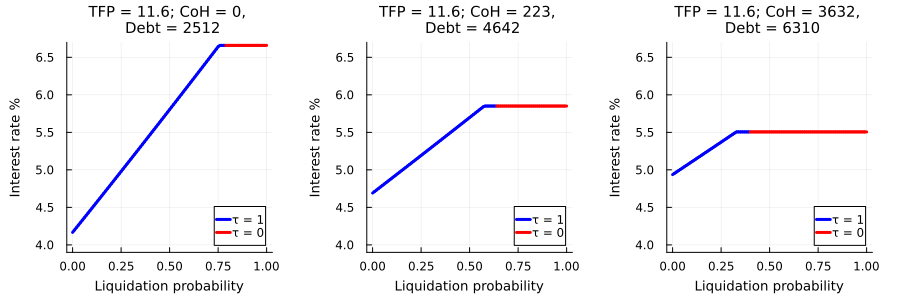
\includegraphics[width=1\textwidth]{Plots/GamPol.png}
    \label{fig:GamPol}
\end{figure} \vspace{-8mm}

\begin{itemize} \small
    \item Liquidation Risk: increases interest rate, decreases CFL reliance
    \item Effects are largest for small but productive firms $\rightarrow $ typically young firms
\end{itemize} \normalsize

\end{frame}


%------------------------------------------------
\begin{frame}[label=tilesplot] \frametitle{The Effects of Reorganization Costs - Firm Effects \hfill \hyperlink{distplot}{\beamergotobutton{Back}}}

\begin{figure}[h!]
    \centering
    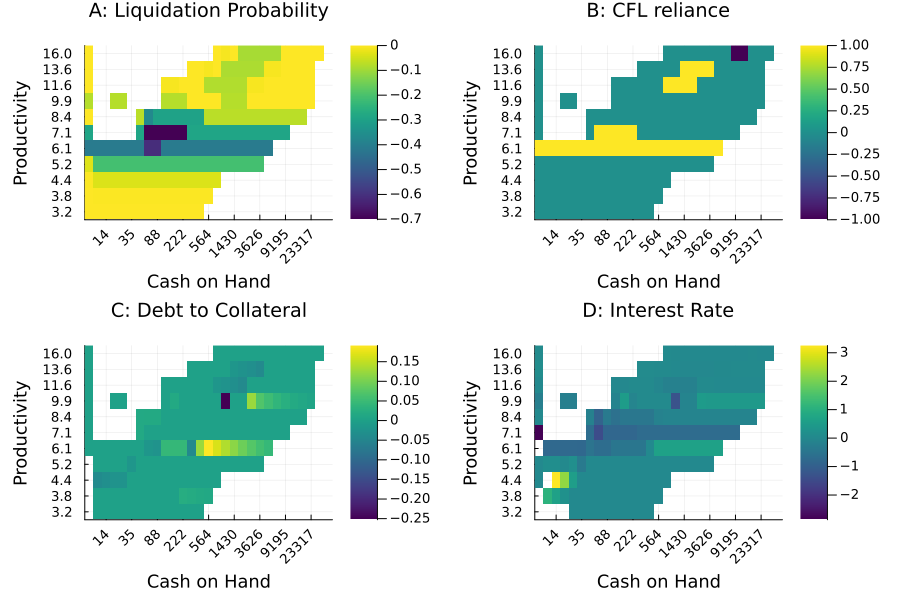
\includegraphics[width=0.8\textwidth]{Plots/reform.png}
    \label{fig:GamPol}
\end{figure}


\end{frame}

%------------------------------------------------
\begin{frame}[label=daysin111] \frametitle{Days in Chapter 11 over Total Assets\hfill \hyperlink{FCreorg}{\beamergotobutton{Back}}}


\begin{figure}[h!]
    \centering
    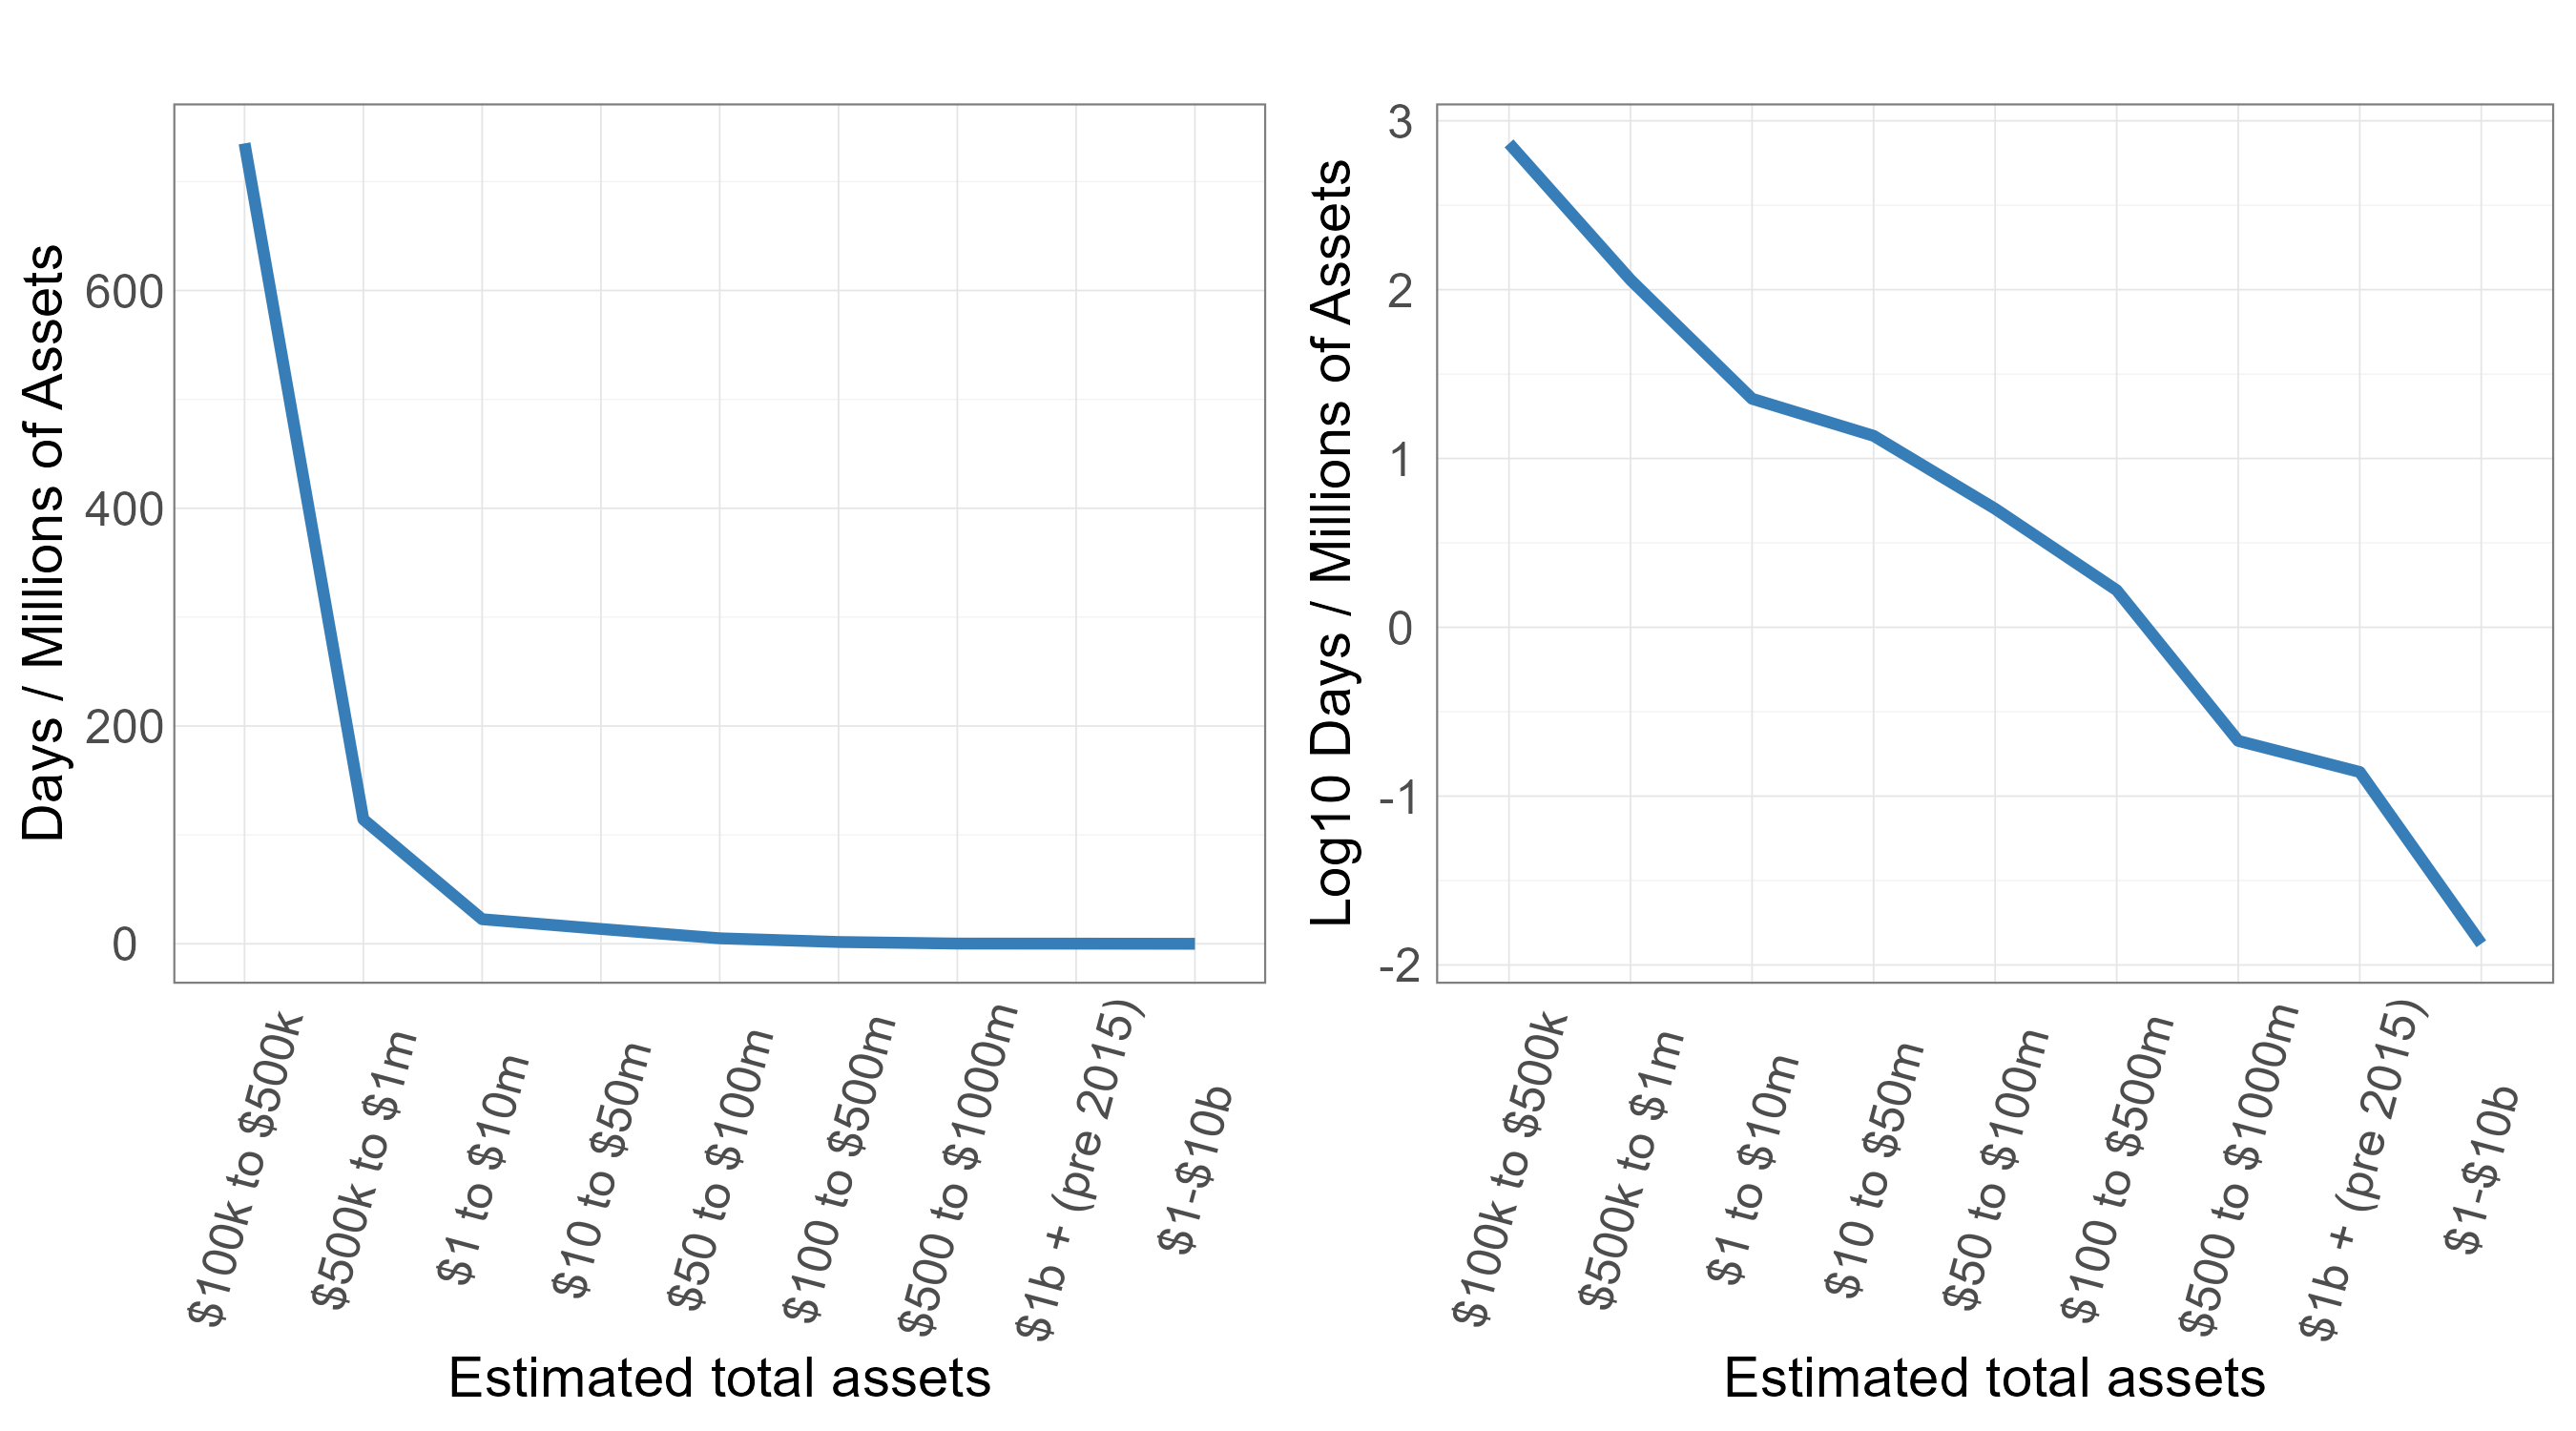
\includegraphics[width=0.9\textwidth]{Plots/daysin11.png}
\end{figure}


\end{frame}


%------------------------------------------------
\begin{frame}[label = SBRA]  \frametitle{The Small Business Reorganization Act \hfill \hyperlink{EUandUS}{\beamergotobutton{Back}}}

Small Business Reorganization Act (effective of February 2020)
\begin{itemize} \small
    \item Reorganization often too expensive for small firms 
    \item Streamlines reorg. process up to a debt limit of \$3M  (\$7.5M under CARES) 
\end{itemize} \normalsize 

Several provisions 
\begin{itemize} \small
    \item Simplified disclosure requirements and faster confirmation timeline
    \item Appointment of a \textit{Subchapter~V Trustee} to aid negotiations
    \item Debtors retain exclusive right to file plans (no creditor proposals)
    \item Easier creditor cramdown and relaxed Absolute Priority Rule (APR)
\end{itemize} \normalsize 

I focus on two features
\begin{itemize} \small
    \item \textbf{Size-based} reduction of reorganization costs
    \item \textbf{Weaker creditor control} over the reorganization process
\end{itemize} \normalsize

\end{frame}

%------------------------------------------------
\begin{frame}[label=sbra_effect] \frametitle{Estimating the SBRA’s Effect}

Back of the envelope calculations based on Hotchkiss, Iverson, and Zheng (2024): 
\begin{itemize} \small
    \item Liquidation probability for small firms drops by approx. 13\%  \hfill \hyperlink{sbra_data}{\beamergotobutton{Details}} 
\end{itemize} \normalsize

Model implementation:
\begin{itemize}\small
    \item A \textbf{targeted cut} in the fixed reorganization cost: \hspace{1.76cm} $\zeta_{small} \rightarrow 0.74\,\zeta$
    \item Compared with: \textit{(i)} universal cost cut; \hspace{3.3cm} $\zeta \rightarrow 0.74\,\zeta$ \\
    \hspace{2.3cm} \textit{(ii)} cost cut \textit{and} reduction in creditor control  $\zeta \rightarrow 0.74\,\zeta$,   $\theta \rightarrow 0.74\,\theta$  
\end{itemize} \vspace{2mm}

\pause

\small
\begin{table}[H]
    \centering
    \renewcommand{\arraystretch}{0.9}
    \begin{tabular}{lccc}
    \textbf{Policy} &  \textbf{Targeted} & \textit{(i)} \textbf{Universal} & \textit{(ii)} \textbf{Control Reduc.} \\    
    \toprule
    Productivity (Y/L) change & 0.81\%  & 0.93\% & -0.54\%  \\  
    \end{tabular}
    \label{tab:percentage_changes2}
\end{table} \normalsize \vspace{2mm}

The SBRA has a meaningful positive effect on productivity: \hfill \hyperlink{sbra_fullres}{\beamergotobutton{Details}} 
\begin{itemize} \small
    \item The size-based policy achieves nearly the full gain
    \item Provisions that reduce creditor may offset these effects
\end{itemize}

\end{frame}



%------------------------------------------------
\begin{frame}[label=sbra_data] \frametitle{Back of the Envelope: SBRA and Liqudation Risk \hfill \hyperlink{EUandUS}{\beamergotobutton{Back}}}

Complicated by the SBRA's overlap with COVID-19 and major policy interventions

\textbf{Hotchkiss, Iverson, and Zheng, 2024:}
\begin{itemize}\small
    \item Combine PACER, LexisNexis, and FJC data 
    \item Use OLS and quasi-experimental methods; I rely on the OLS estimate  
    \item SBRA increases plan confirmation by about \textbf{21 pp}  
          (from 32.9 \% to roughly 54.9 \%)
\end{itemize}
\vspace{3mm}

\textbf{IDB data}: for eligible firms, the prob. of filing for CH11 increases from 0.471 to 0.520 

\textbf{Back-of-the-envelope calculation:}
\[
\begin{aligned}
\text{2019 (pre-SBRA):}\;& 0.471 \times 0.329 = 0.155 \Rightarrow 84.5\% \text{ liquidation} \\
\text{2024 (post-SBRA):}\;& 0.520 \times 0.549 = 0.285 \Rightarrow 71.5\% \text{ liquidation}
\end{aligned}
\]

\end{frame}


%------------------------------------------------
\begin{frame}[label=sbra_emp] \frametitle{Changes in Liquidation Risk and CF-reliance - 2010-2024  \hfill \hyperlink{EUandUS}{\beamergotobutton{Back}}}

\begin{columns}[T,onlytextwidth]
  \begin{column}{0.46\textwidth}
    \centering
    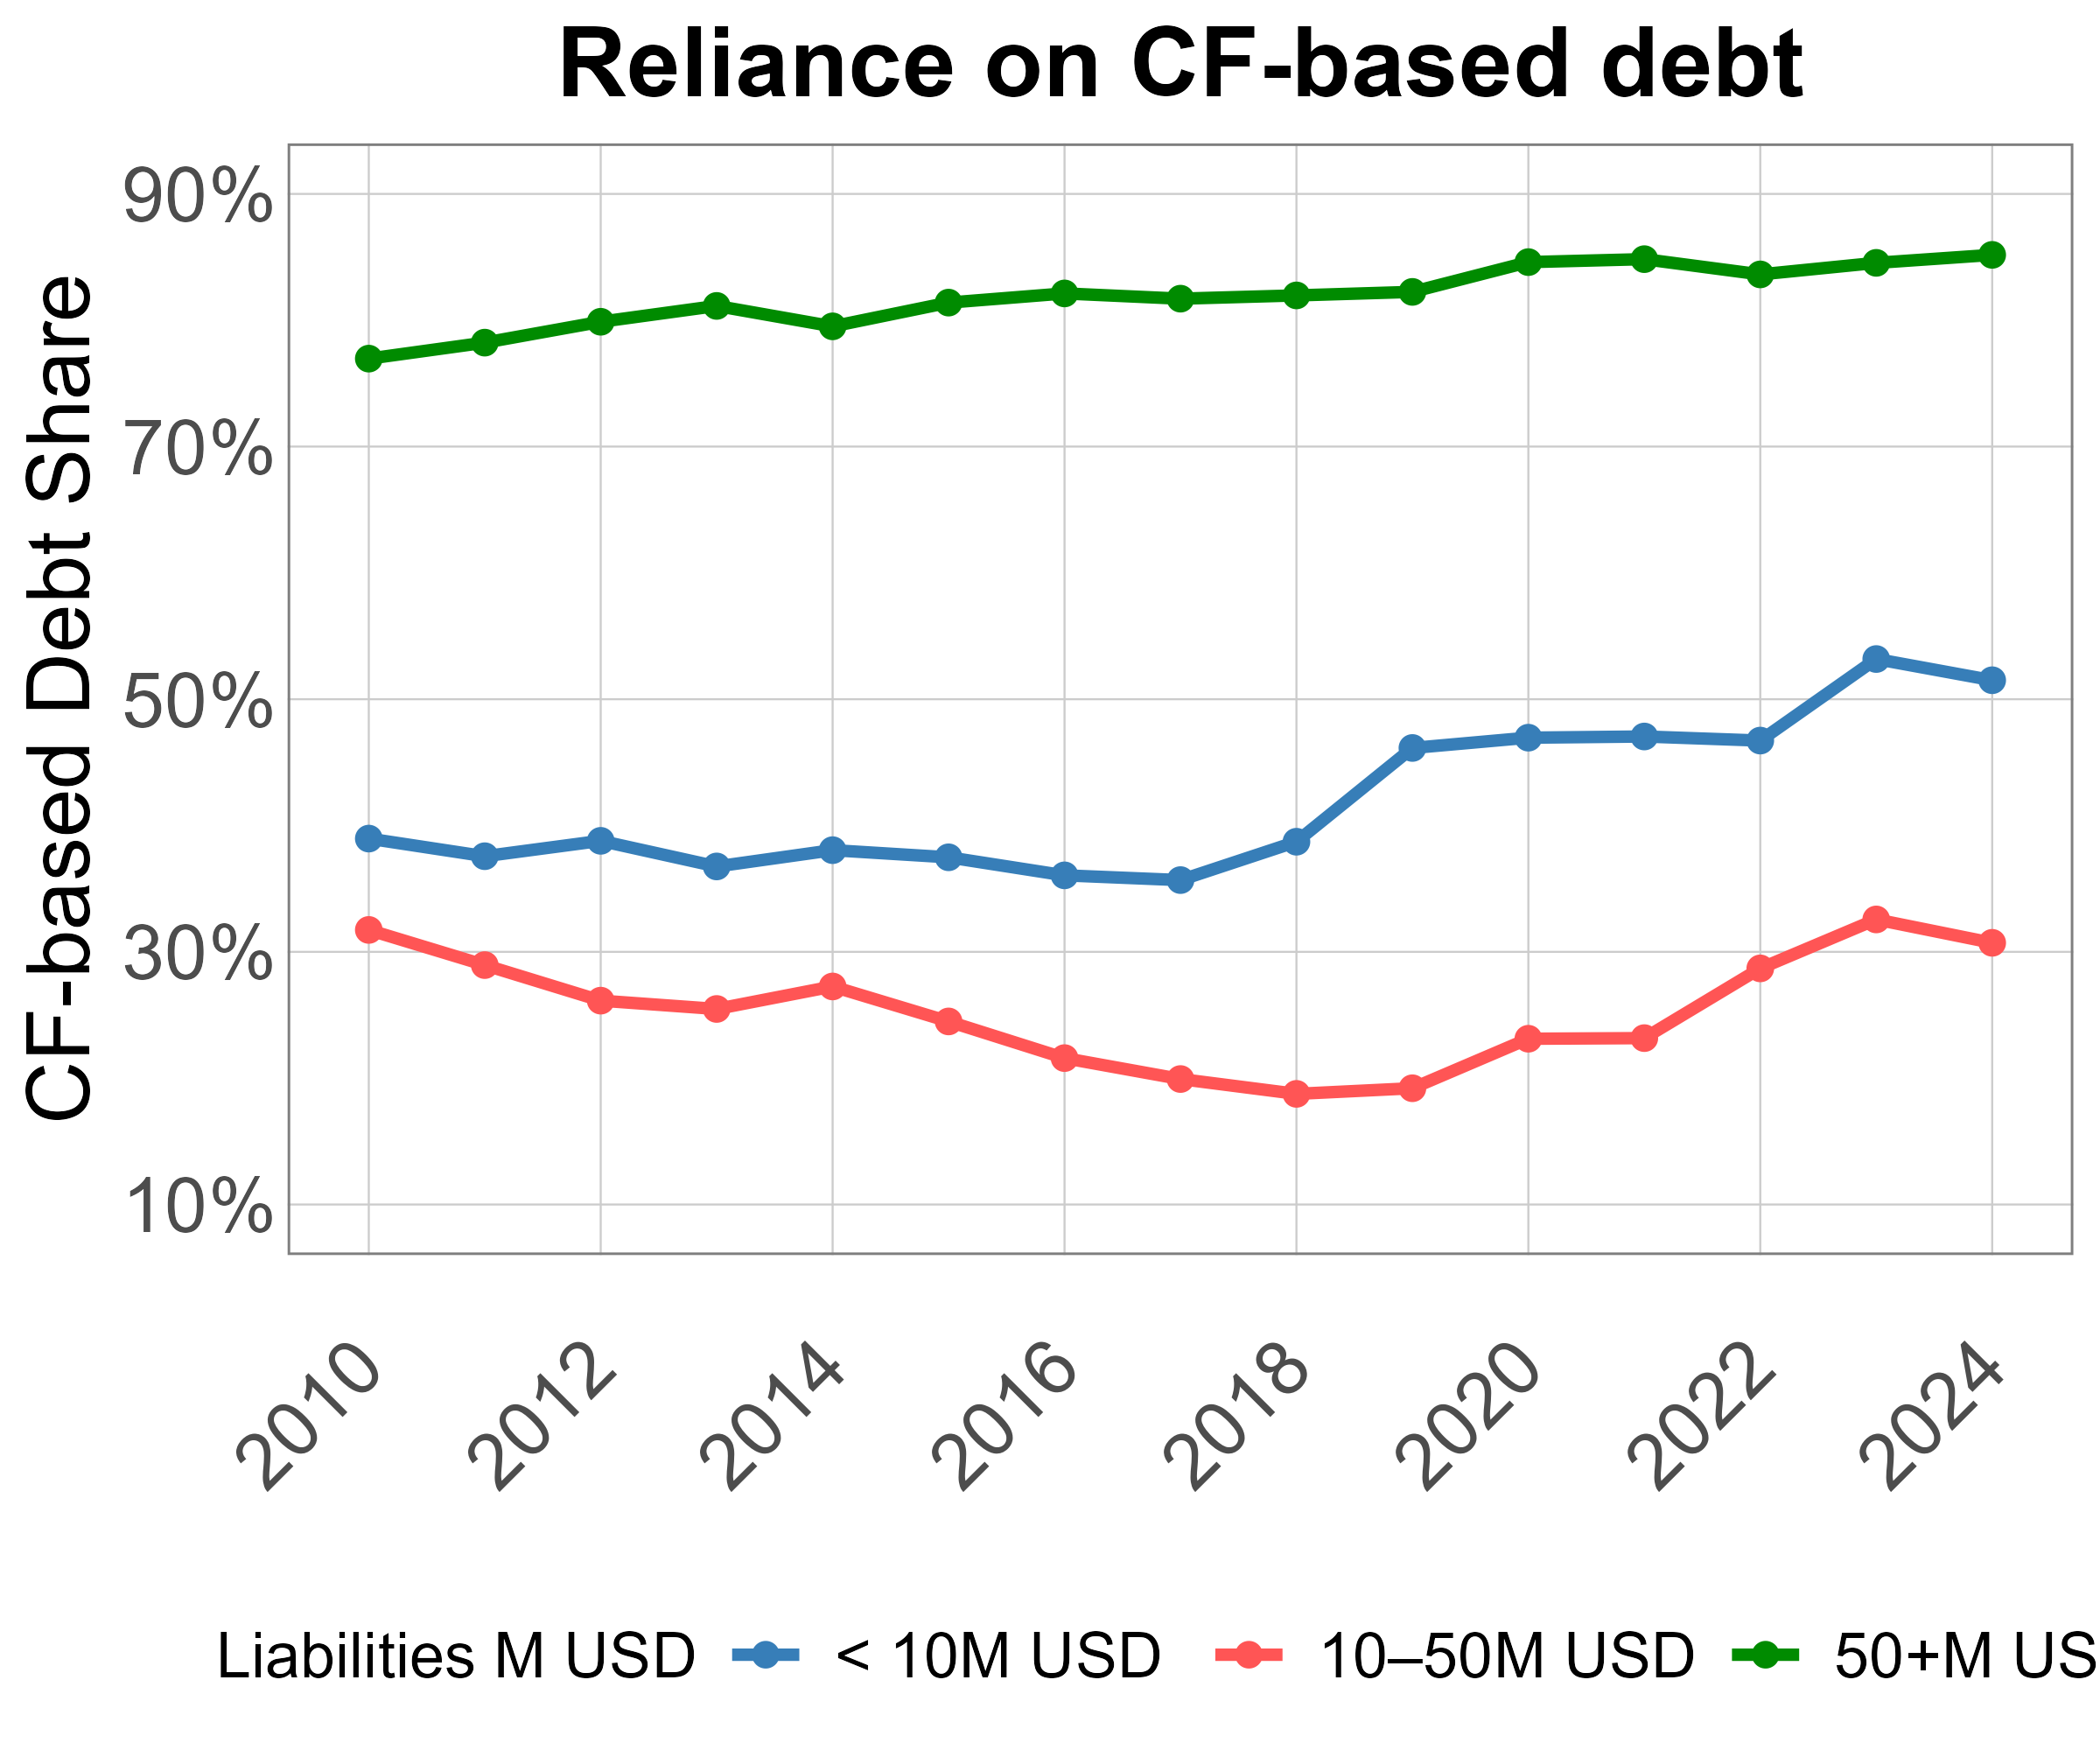
\includegraphics[width=\textwidth]{Plots/CFshare_firms.png}
    \vspace{0.2cm}
  \end{column}

  \begin{column}{0.46\textwidth}
    \centering
    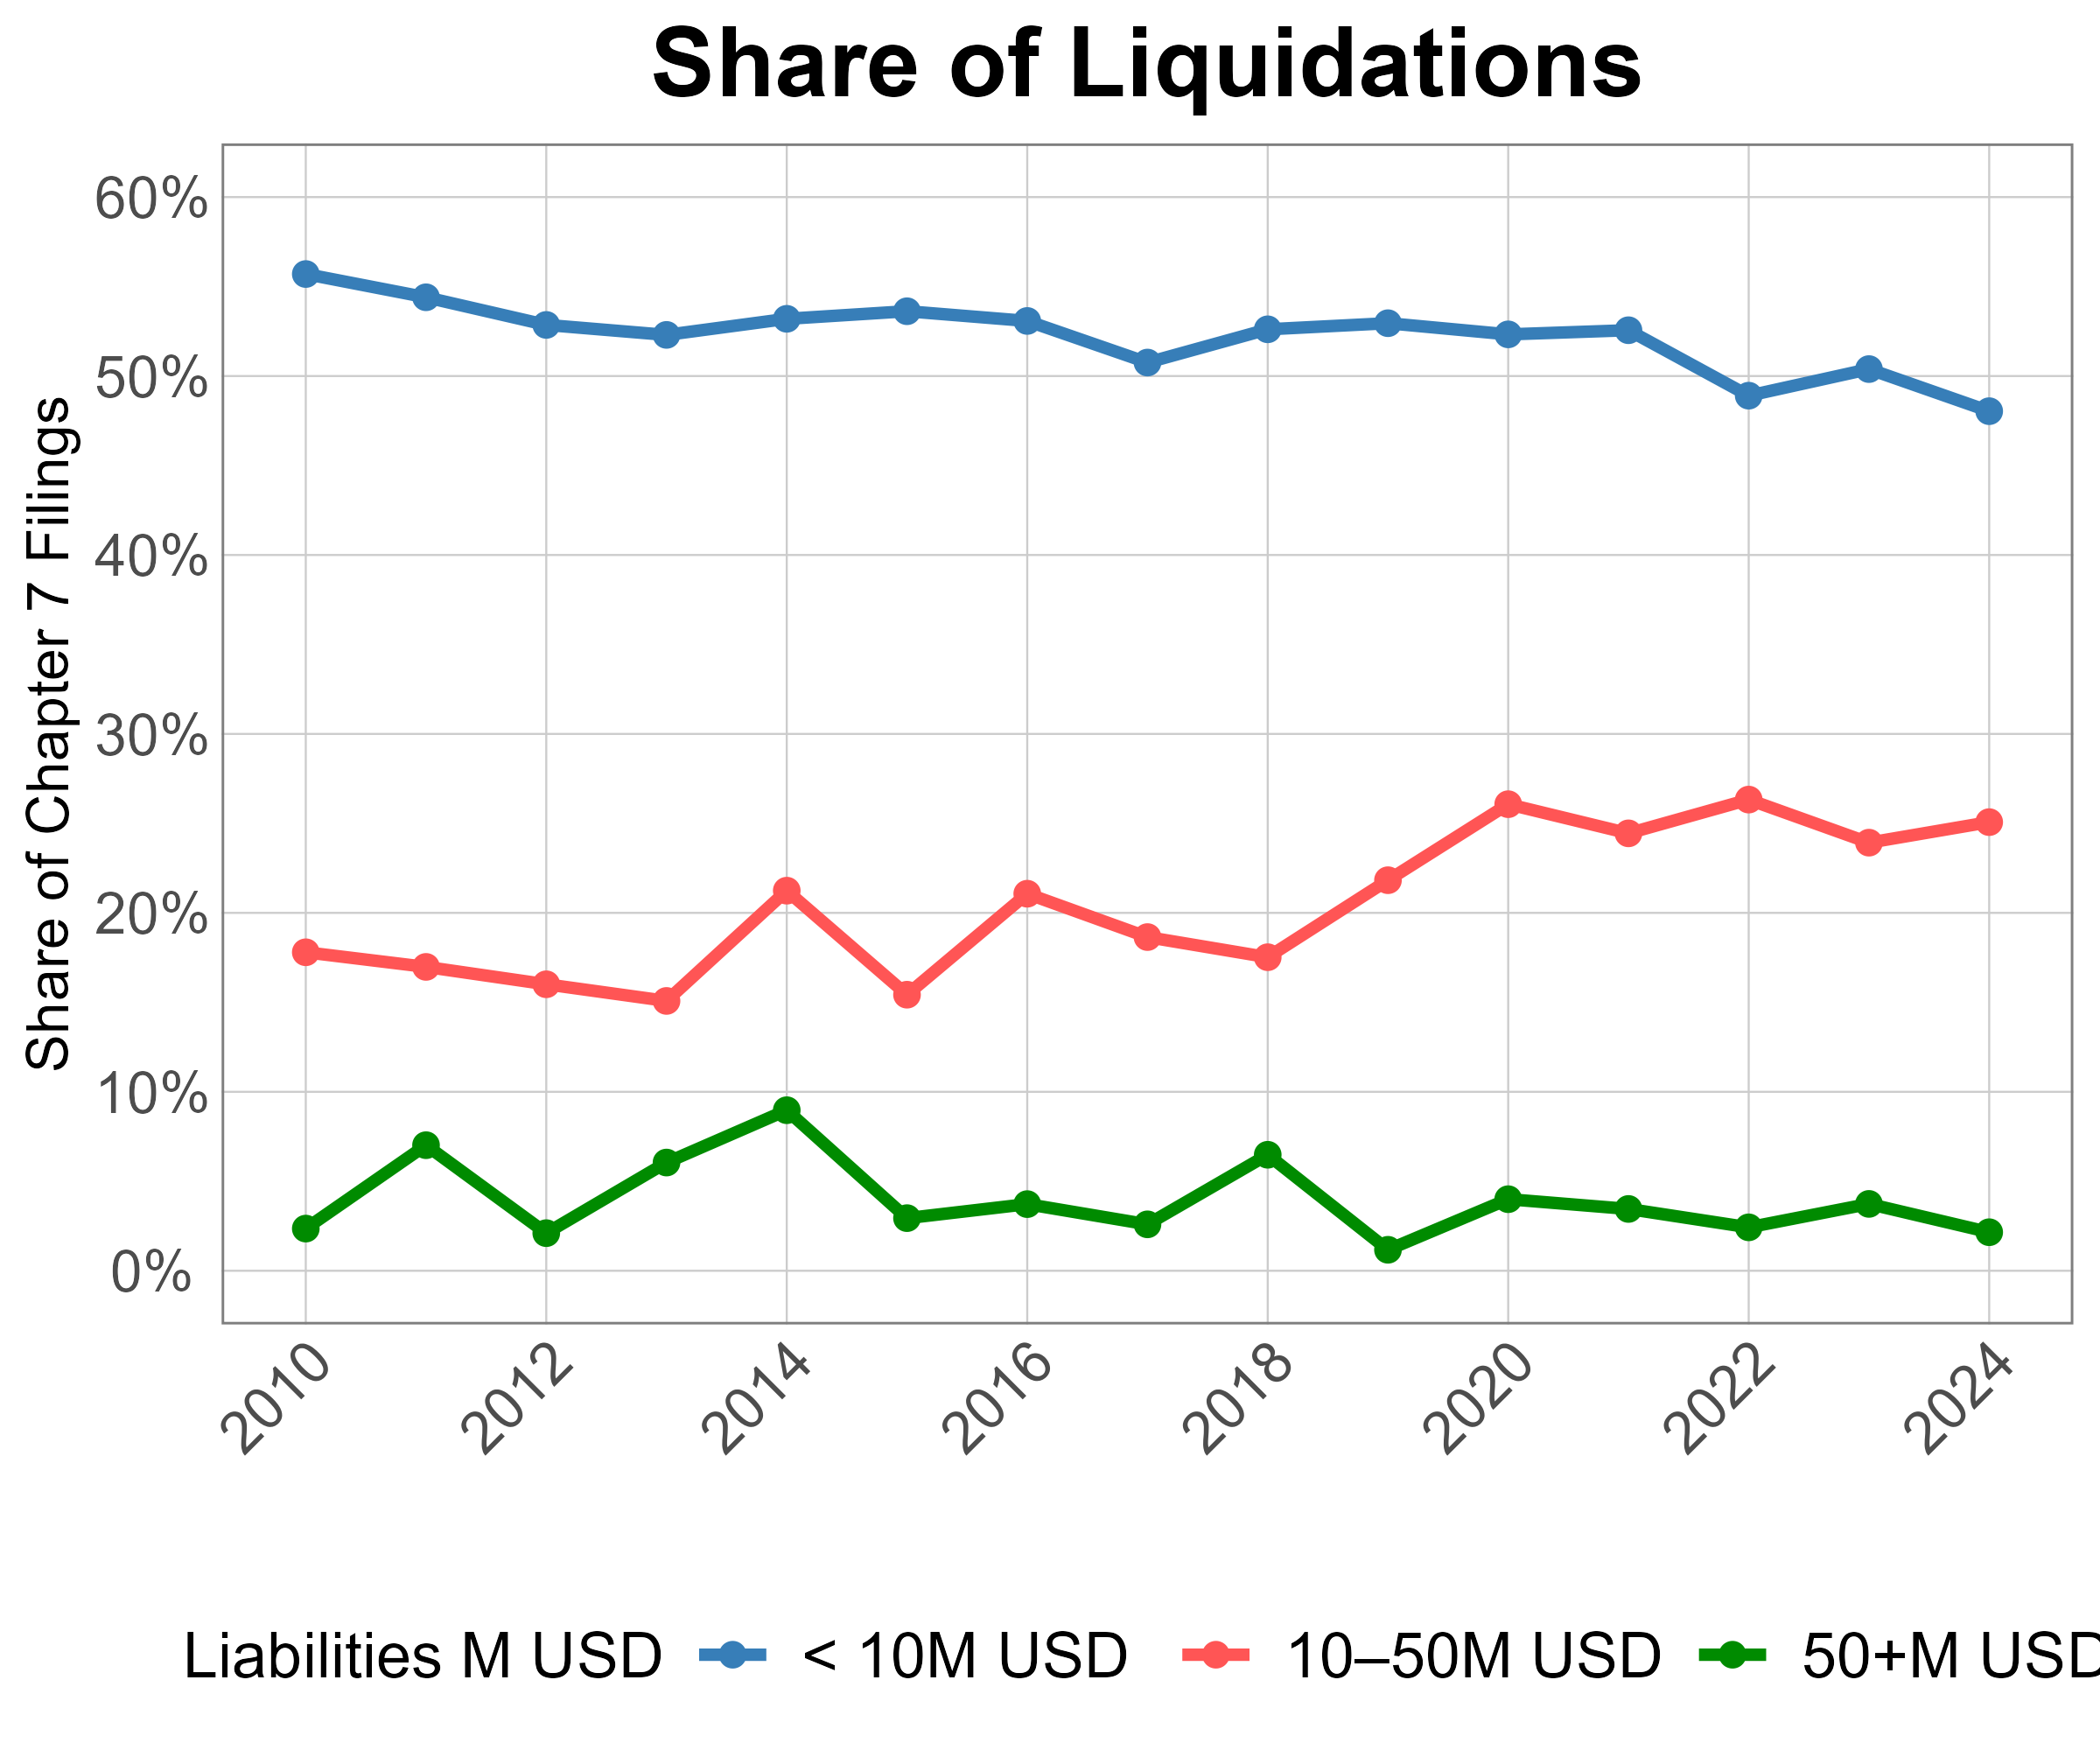
\includegraphics[width=\textwidth]{Plots/Liqprob_OT.png}
    \vspace{0.2cm}
  \end{column}
\end{columns}

\vspace{-5mm}

\begin{itemize}\small
  \item Liquidation risk falls and reliance on CF-based debt increases around 2020
  \item The extent to which this is attributable to the SBRA is unclear
\end{itemize}

\end{frame}


%------------------------------------------------
\begin{frame}[label=sbra_emp] \frametitle{Callaway and Sant’Anna (2021) DiD Estimator \hfill \hyperlink{EUandUS}{\beamergotobutton{Back}}}

\centering
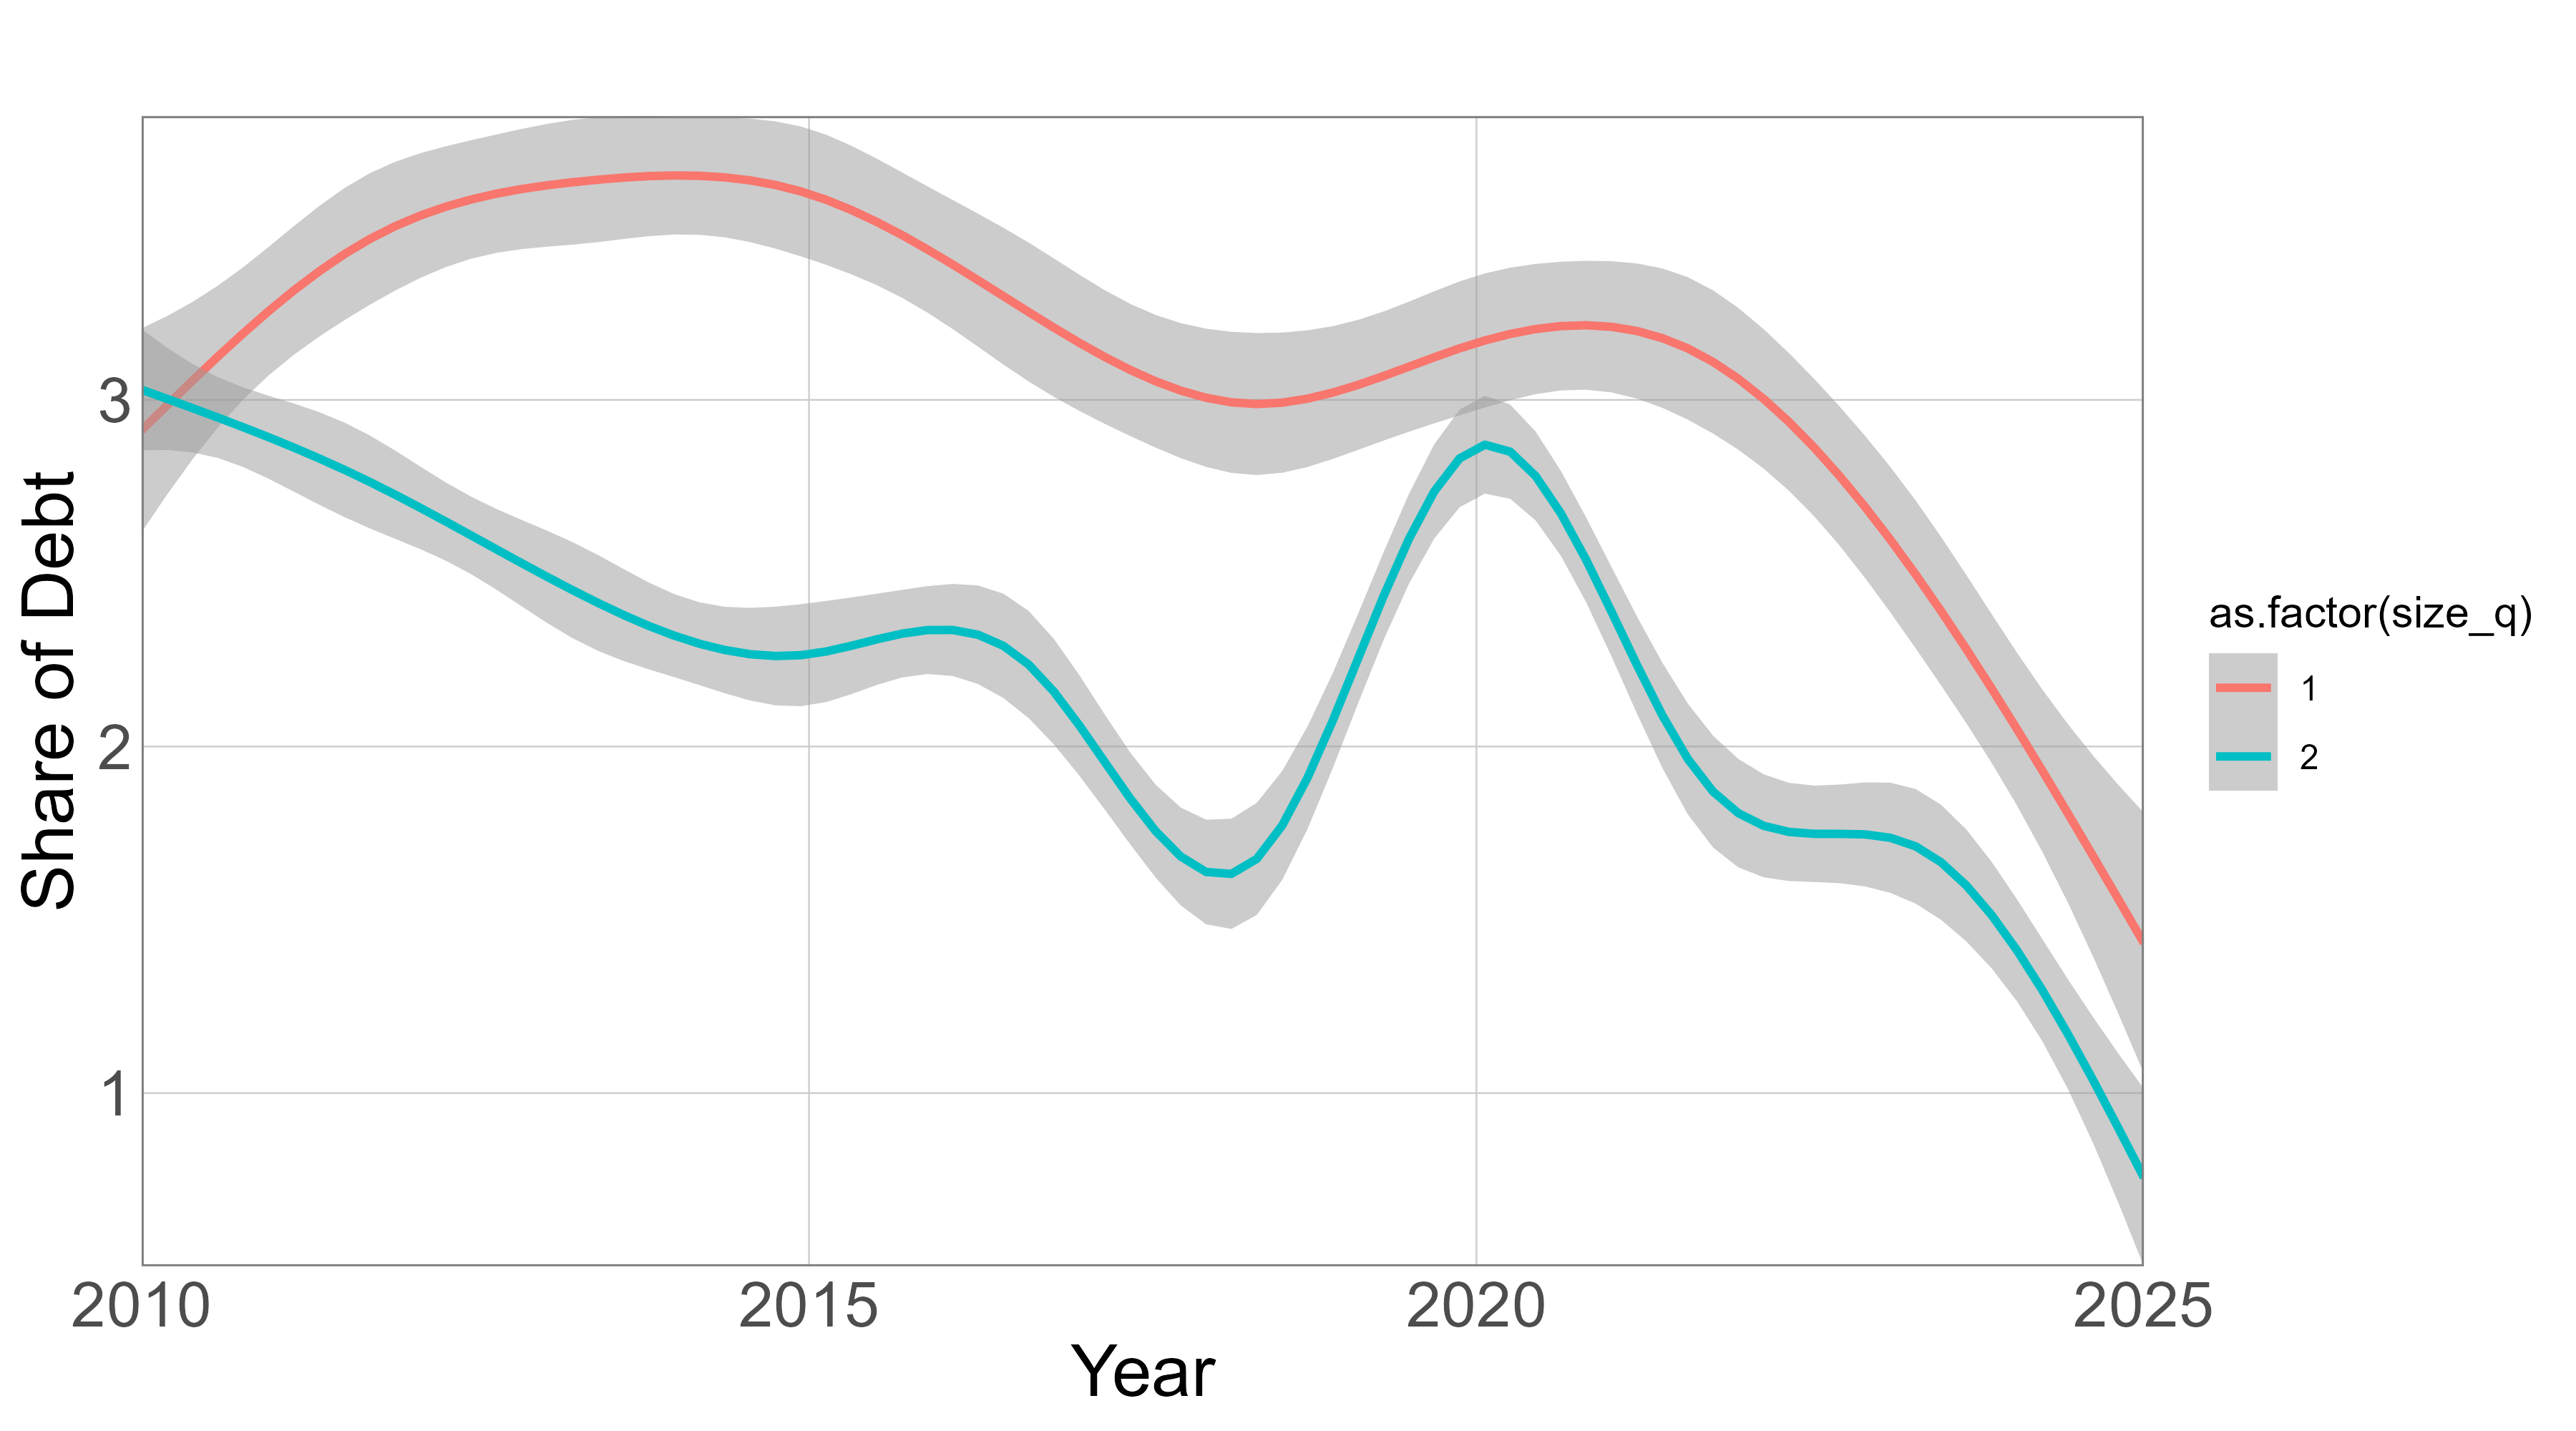
\includegraphics[width=1\textwidth]{Plots/DID.png}



\end{frame}


\end{document}
